\chapter{実験}
\label{chap:ex}

%----------------------------------------------
\section{まえがき}
%----------------------------------------------
前章で提案したDNNに基づくパーミュテーション解決法の有効性を確認するために,人工的に作成したデータと実際の音声及び音楽信号を用意し,提案パーミュテーション解決法を適用する.後に,その性能を評価した.
\ref{sec:ex_condition}節では,本実験における条件を詳細に示し,\ref{sec:ex_res}節では提案手法のパーミュテーション解決性能を示している.
\ref{sec:matome}節で本章のまとめを述べる.
%----------------------------------------------
\section{実験条件}
\label{sec:ex_condition}
%----------------------------------------------
% \begin{table}[t]
% \begin{center}
%  \caption{Experimental conditions}
%  \label{table:ex}
%   \begin{tabular}{clll}\hline \hline
%    Window function in STFT & Hamming window  \\ \hline
%    Window length in STFT & 512~ms  \\ \hline
%    Shift length in STFT & 128~ms \\ \hline
%    Paramaters in Adam optimizer & \begin{tabular}{c}
%    \begin{flushleft}Learning rate = $0.001$\end{flushleft}\\
%    \begin{flushleft}$\beta = 0.9$\end{flushleft}
%    \end{tabular}  \\ \hline 
%    Reverberation time & $T_{60} = 470$~ms\\ \hline
%    Source direction of training data & $(\theta_1, \theta_2)=(60^\circ, 120^\circ)$\\ \hline
%    Source direction of test data & \begin{tabular}{c}
%    \begin{flushleft}(\theta_1, \theta_2)=(60^\circ, 120^\circ)\end{flushleft}\\ 
%    \begin{flushleft}(\theta_1, \theta_2)=(60^\circ, 100^\circ)\end{flushleft}\\ 
%    \begin{flushleft}(\theta_1, \theta_2)=(70^\circ, 110^\circ)\end{flushleft}
%    \end{tabular}\\ \hline \hline
%   \end{tabular}
%  \end{center}
% \end{table}
本実験では,提案するDNNに基づくパーミュテーション解決法において,どの程度各周波数成分の並び替えができるかを実験的に確認した.
実験には,人工データと実際の音声及び音楽信号を用いた.
%----------------------------------------------
\subsection{人工データを用いた実験の条件}
\label{sec:ex_condition_matrix}
%----------------------------------------------
実験データとして,Fig.~\ref{fig:01mat_spec}--\ref{fig:stripe_spec}に示すように,全ての成分が0と1の行列,25列毎に0と1の値が入れ替わる行列,1列毎に0と1の値が入れ替わる行列の3パターンを使用した.
用意した3パターンの行列は,いずれもパーミュテーション問題が生じていない(完全に解決された状態の)分離信号$(\bm{Z}_1, \bm{Z}_2)$とみなして実験を行う.この時の行列のサイズは$I=J=100$とした.
また,ブロックパーミュテーションと呼ばれる,ブロック単位でのパーミュテーション問題を模擬するために,Fig.~\ref{fig:ex_block}のように2行,4行,8行毎に各周波数成分を音源間でランダムにシャッフルした行列を作成し,
これをパーミュテーション問題が生じている(未解決の)信号$(\bm{Y}_1, \bm{Y}_2)$の検証データ及びテストデータとみなして深層パーミュテーション解決法の入力に用いた際の性能を評価した.
Fig.~\ref{fig:stripe_spec}に示す1列毎に0と1の値が入れ替わる行列に対しては,5\%の割合で2行毎にシャッフルしそれ以外は1行毎にシャッフルした場合と,1\%の割合で2行毎にシャッフルしそれ以外は1行毎にシャッフルした場合の実験も行った.

\begin{figure}[htbp]
    \begin{minipage}[b]{0.45\linewidth}
      \centering
      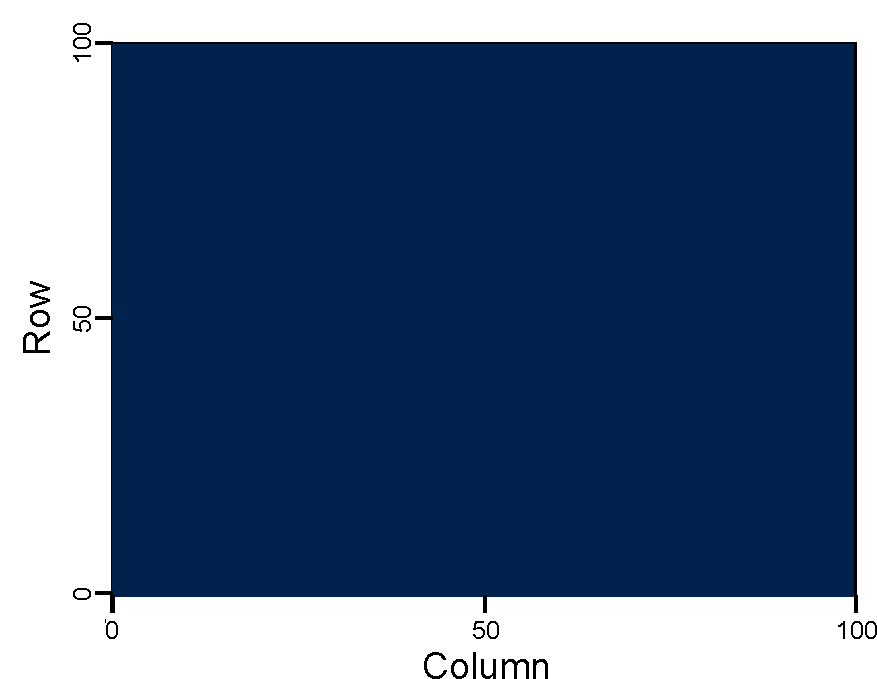
\includegraphics[keepaspectratio, width=6.0cm]{figures/origi_spec/0mat.pdf}
    \end{minipage}
    \begin{minipage}[b]{0.45\linewidth}
      \centering
      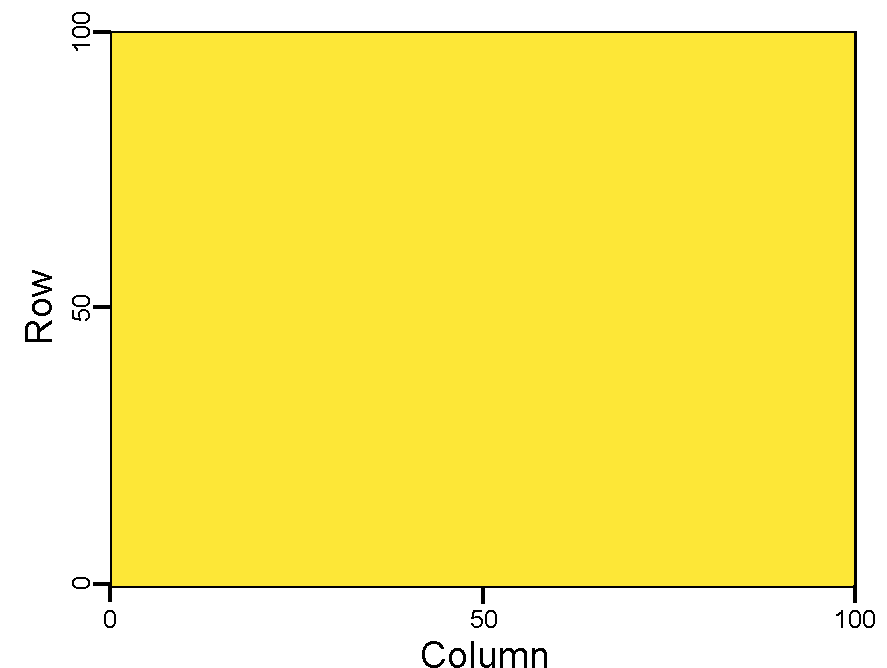
\includegraphics[keepaspectratio, width=6.0cm]{figures/origi_spec/1mat.pdf}
    \end{minipage}
    \caption{Matrix with only 0 or 1 elements.}
    \label{fig:01mat_spec}
\end{figure}

\begin{figure}[htbp]
    \begin{minipage}[b]{0.45\linewidth}
      \centering
      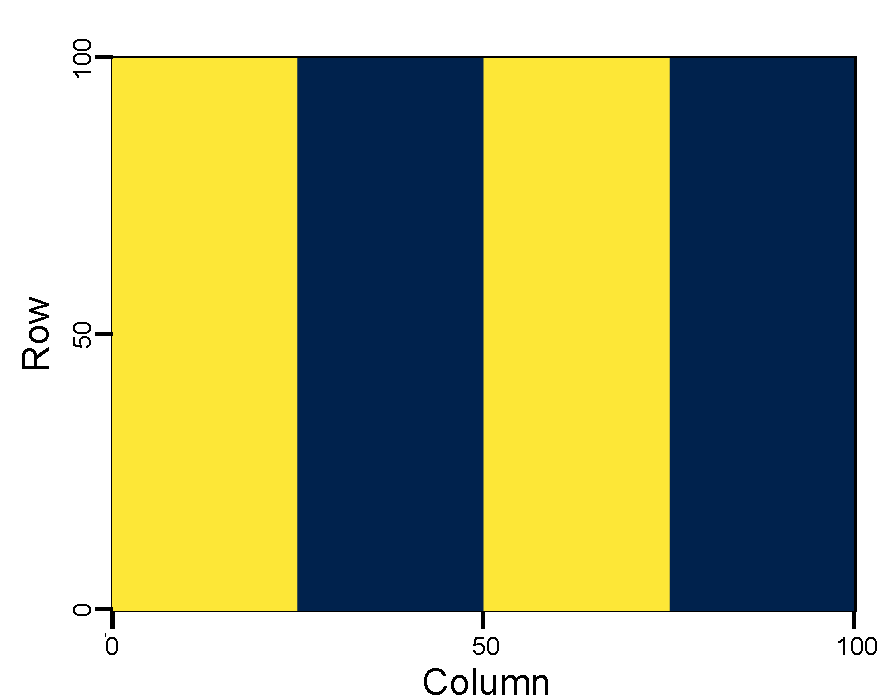
\includegraphics[keepaspectratio, width=6.0cm]{figures/origi_spec/25stripe1.pdf}
    \end{minipage}
    \begin{minipage}[b]{0.45\linewidth}
      \centering
      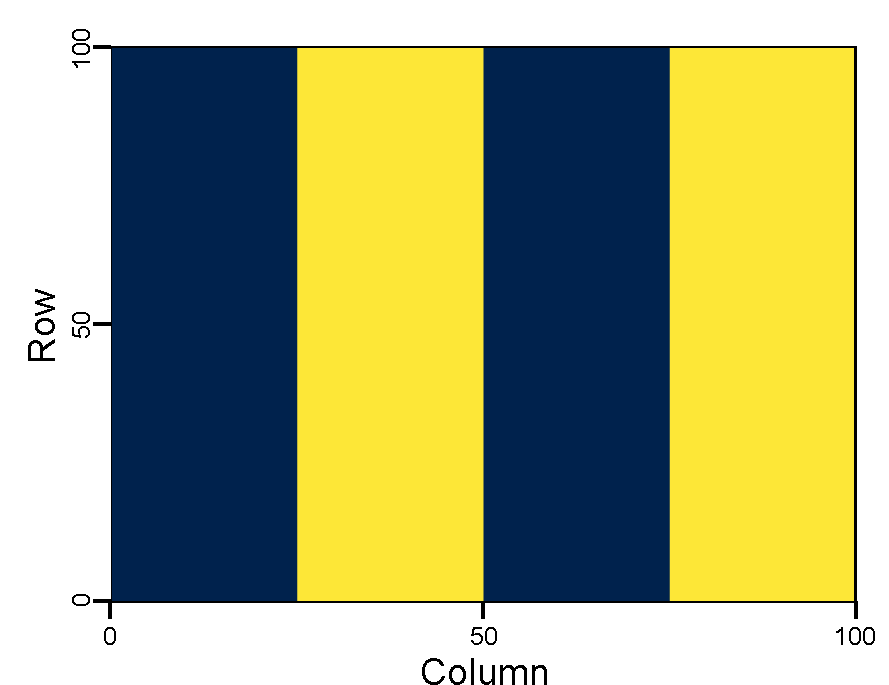
\includegraphics[keepaspectratio, width=6.0cm]{figures/origi_spec/25stripe2.pdf}
    \end{minipage}
    \caption{Two matrices with 0 and 1 values swapping every 25 columns.}
    \label{fig:25stripe_spec}
\end{figure}

\begin{figure}[htbp]
    \begin{minipage}[b]{0.45\linewidth}
      \centering
      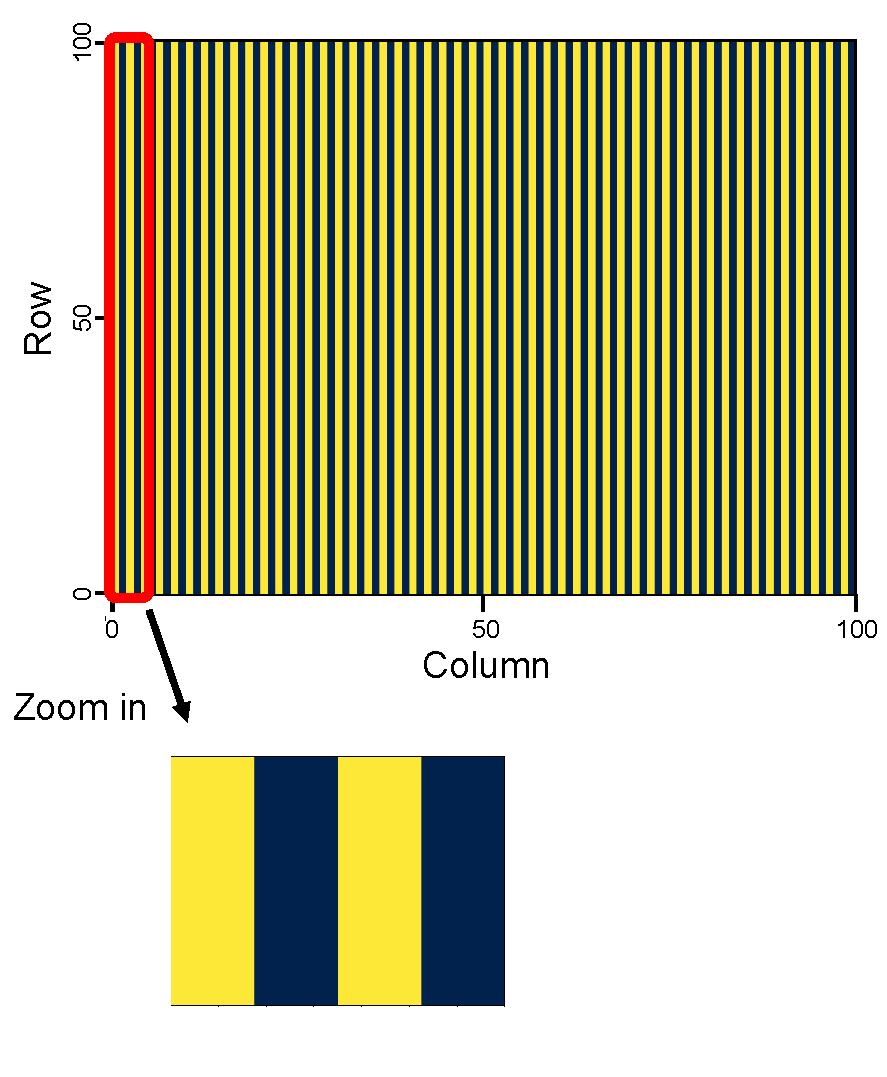
\includegraphics[keepaspectratio, width=6.0cm]{figures/origi_spec/stripe1.pdf}
    \end{minipage}
    \begin{minipage}[b]{0.45\linewidth}
      \centering
      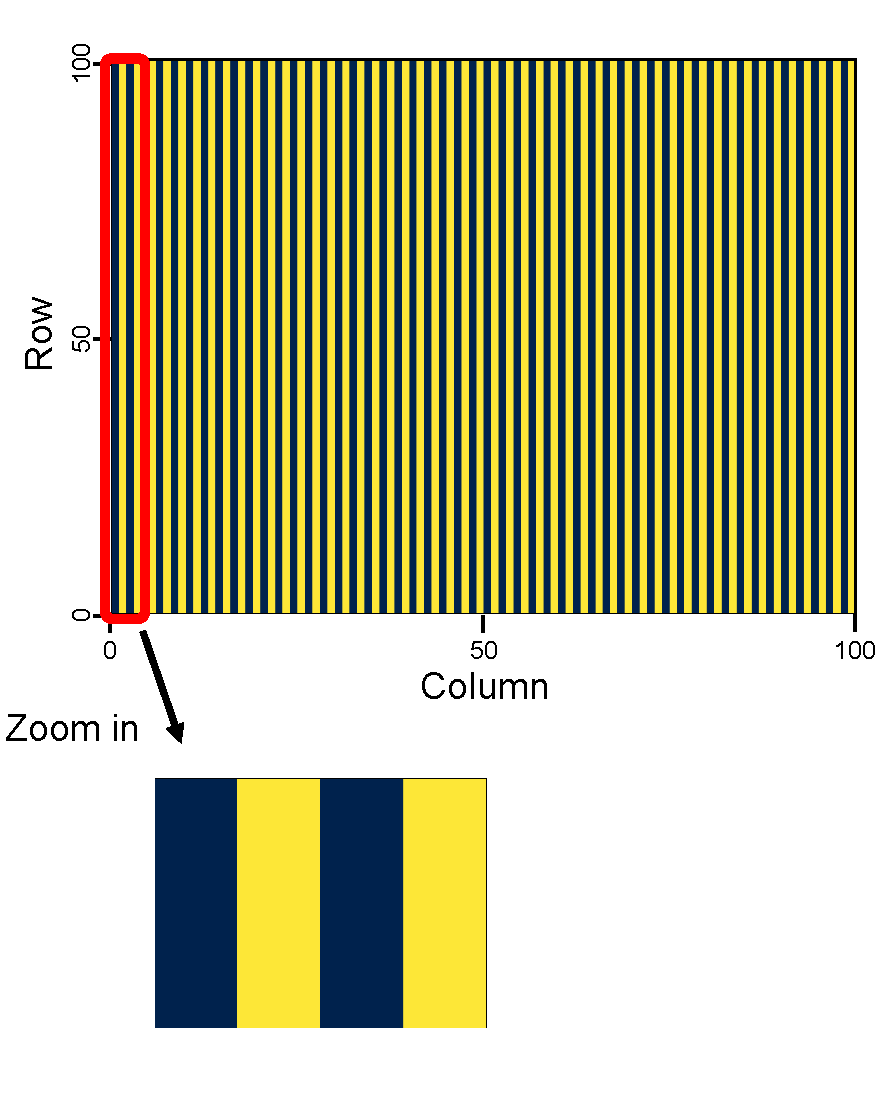
\includegraphics[keepaspectratio, width=6.0cm]{figures/origi_spec/stripe2.pdf}
    \end{minipage}
    \caption{Two matrices with 0 and 1 values swapping in each column.}
    \label{fig:stripe_spec}
\end{figure}

%%%%%%%%%%%%%%%%%%%%%%%%%%%%
\begin{figure}[t]
    \begin{center}
        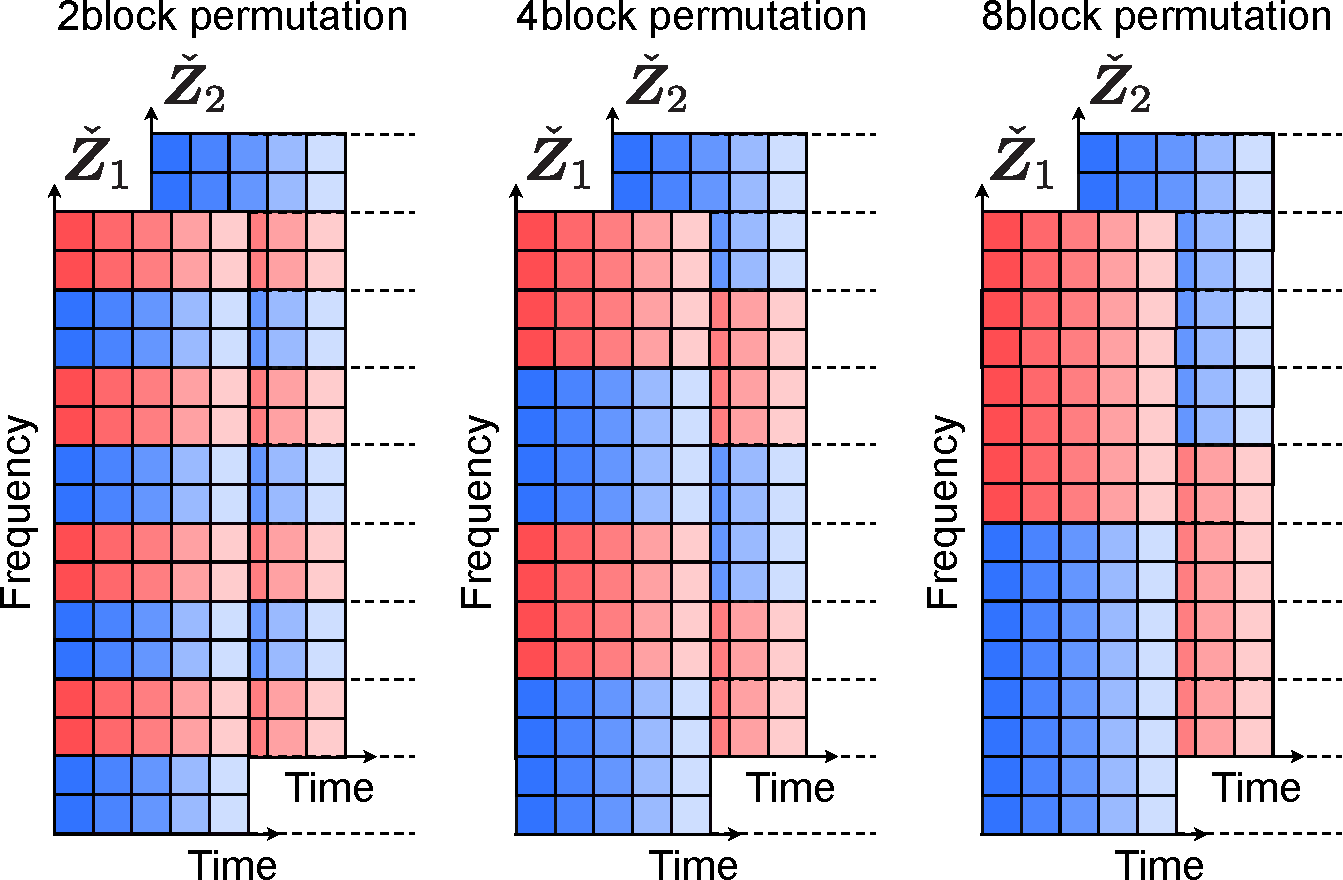
\includegraphics[width=1.0\columnwidth]{figures/experiment_block_matrix.pdf}
    \end{center}
	\caption{Example of block permutations used in the experiment.}
	\label{fig:ex_block}
\end{figure}
%%%%%%%%%%%%%%%%%%%%%%%%%%%%

% %%%%%%%%%%%%%%%%%%%%%%%%%%%%
% \begin{figure}[t]
%     \begin{center}
%         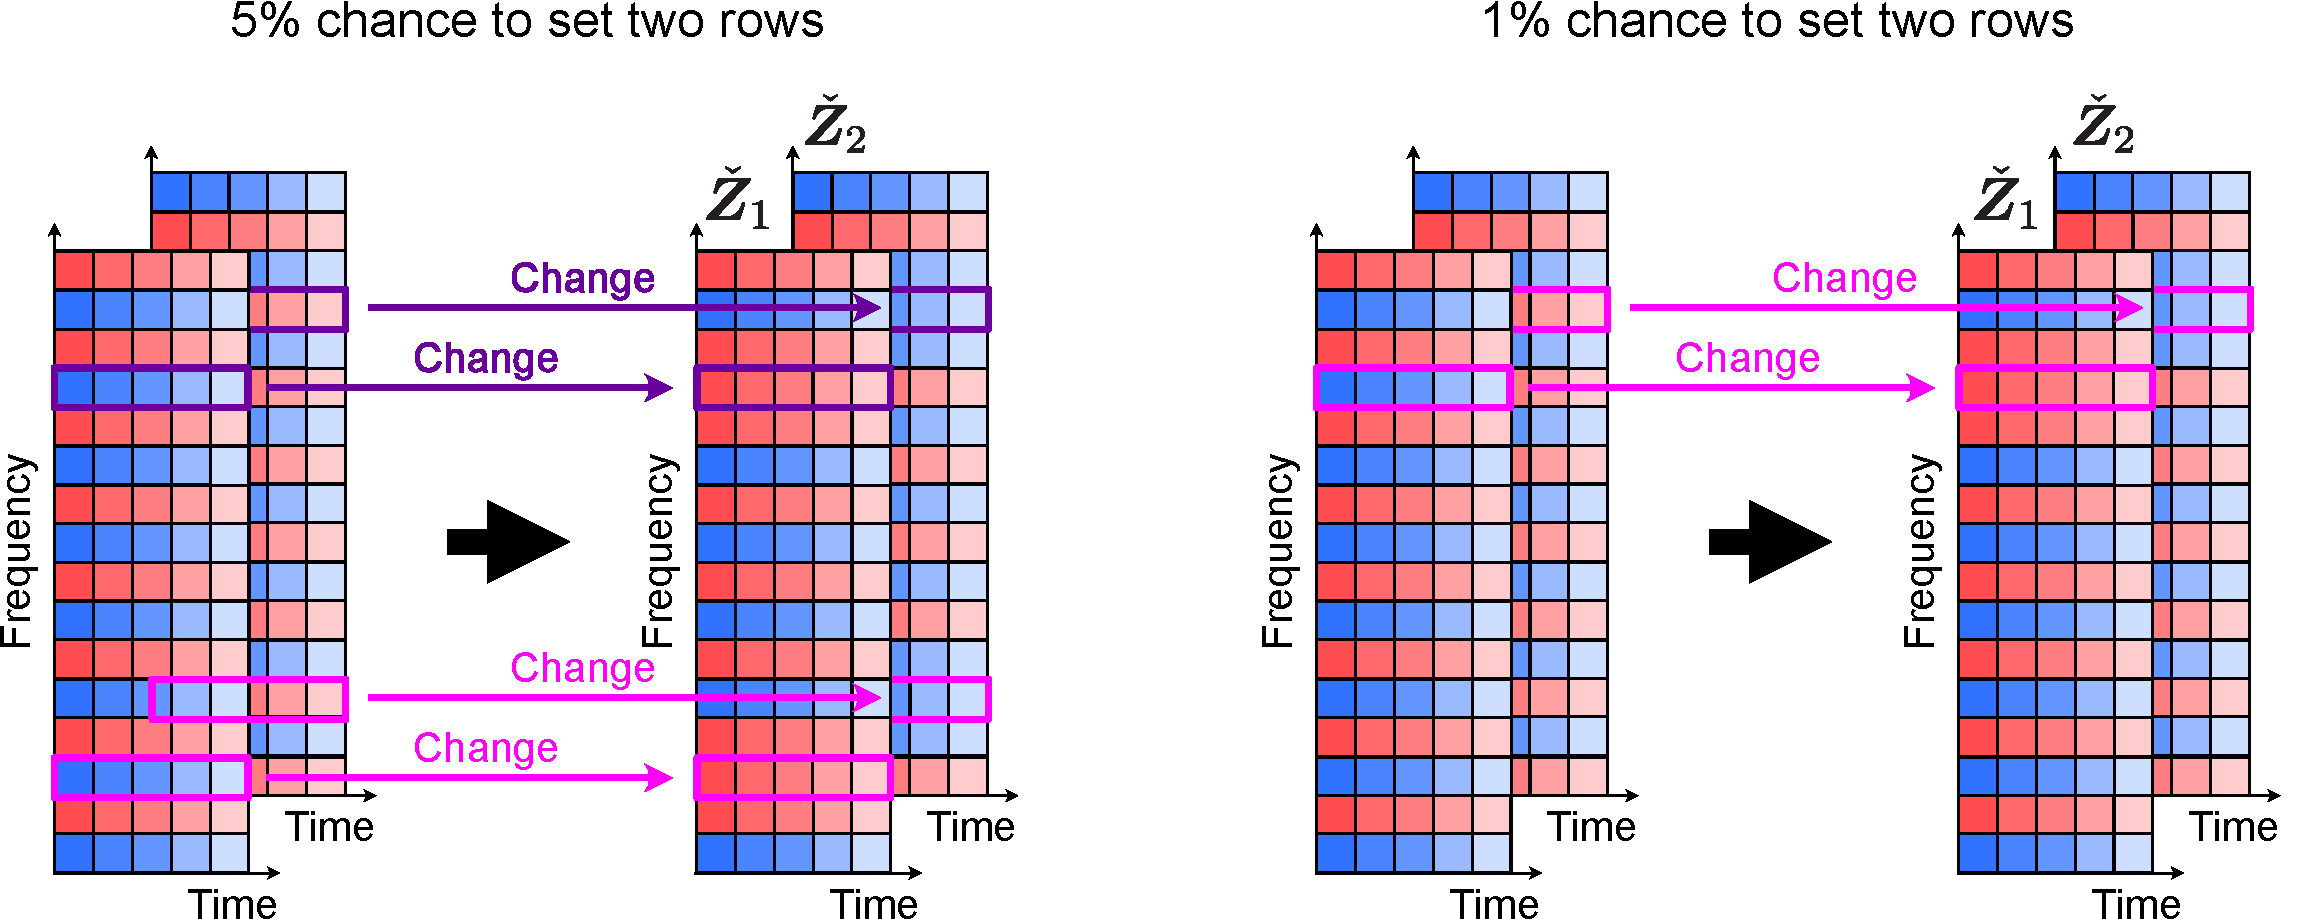
\includegraphics[width=1.0\columnwidth]{figures/1ratio_5ratio_permutation.pdf}
%     \end{center}
% 	\caption{Example of permuting in two blocks according to proportions.}
% 	\label{fig:1_5ratio_perm}
% \end{figure}
% %%%%%%%%%%%%%%%%%%%%%%%%%%%%

学習データには,分離信号の局所時間振幅スペクトログラム$(\check{\bm{Z}}_1, \check{\bm{Z}}_2)$の周波数成分を指定したブロック行毎に音源間でランダムにシャッフルしたものを用いた.
検証データは,学習データには含まれていないシャッフルパターンを用いて$\check{\bm{Z}}_1$と$\check{\bm{Z}}_2$の周波数成分を指定したブロック行毎に音源間でランダムにシャッフルさせることで作成した.
DNNの最適化法にはAdam~\cite{adam}を用い,ハイパーパラメータはそれぞれ$\varepsilon=1.0\times10^{-8},~\beta_1 = 0.9,~\beta_2 = 0.999$及び,学習率$\eta=0.001$とした.
その他の学習パラメータについては,バッチサイズを8,エポック数を1000,学習に用いるシャッフルパターンを300として誤差逆伝搬による学習を行った.
客観評価尺度として,各周波数成分において正しく並び替えを行うことができた割合,即ち検証データに対する正答率を用いる.

%----------------------------------------------
\subsection{実際の音響信号を用いた実験の条件}
\label{sec:ex_condition_audio}
%----------------------------------------------

%----------------------------------------------
\begin{table}[t]
  \begin{center}
   \caption{Speech sources obtained from SiSEC2011}
   \label{table:wav}
    \begin{tabular}{clll}\hline \hline
     Signal  & Data name &Length~[s]  \\ \hline
     Speech  & dev3\_female4\_src\_2 & 11.0  \\ \hline
     Speech  & dev2\_male4\_src\_2 &  11.0 \\ \hline
     Piano   & dev2\_nodrums\_liverec\_250ms\_src\_3 & 12.0\\ \hline
     Drum   & dev2\_wdrums\_liverec\_250ms\_src\_3 & 12.0 \\ \hline 
     \hline
    \end{tabular}
   \end{center}
\end{table}
%%%%%%%%%%%%%%%%%%%%%%%%%%%%
\begin{figure}[t]
  \begin{center}
      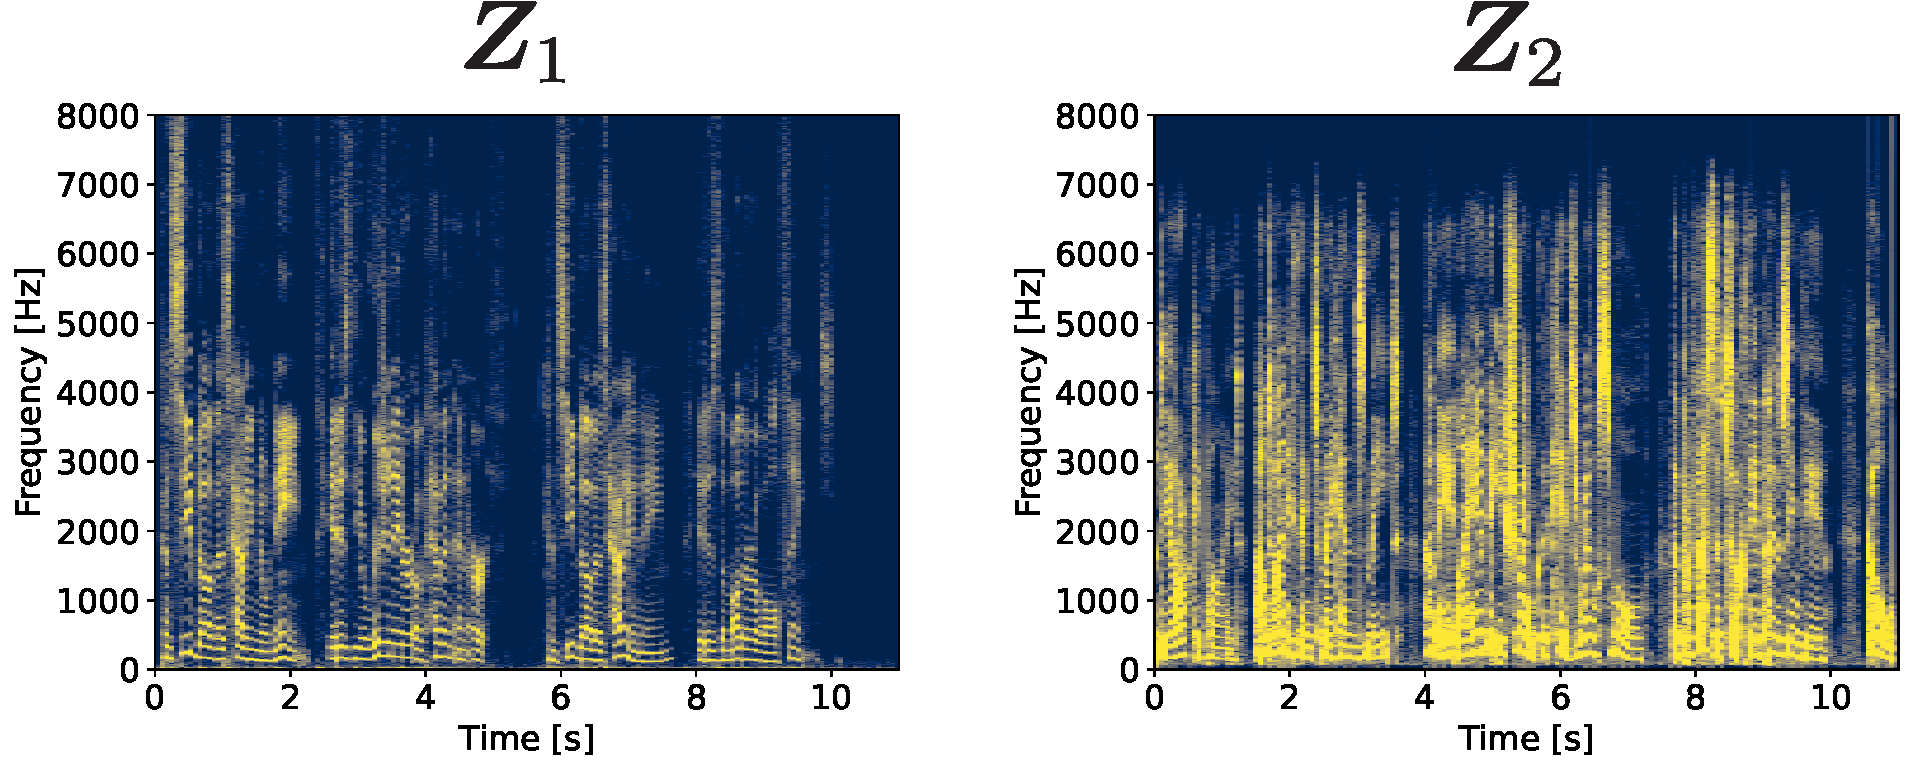
\includegraphics[width=0.95\columnwidth]{figures/audio_init_spec.pdf}
  \end{center}
  \vspace{-8pt}
\caption{Uncertainty in ICA. ICA cannot determine order and scales of estimated signals.}
\label{fig:audio}
\end{figure}
%%%%%%%%%%%%%%%%%%%%%%%%%%%%

%%%%%%%%%%%%%%%%%%%%%%%%%%%%
\begin{figure}[t]
  \begin{center}
      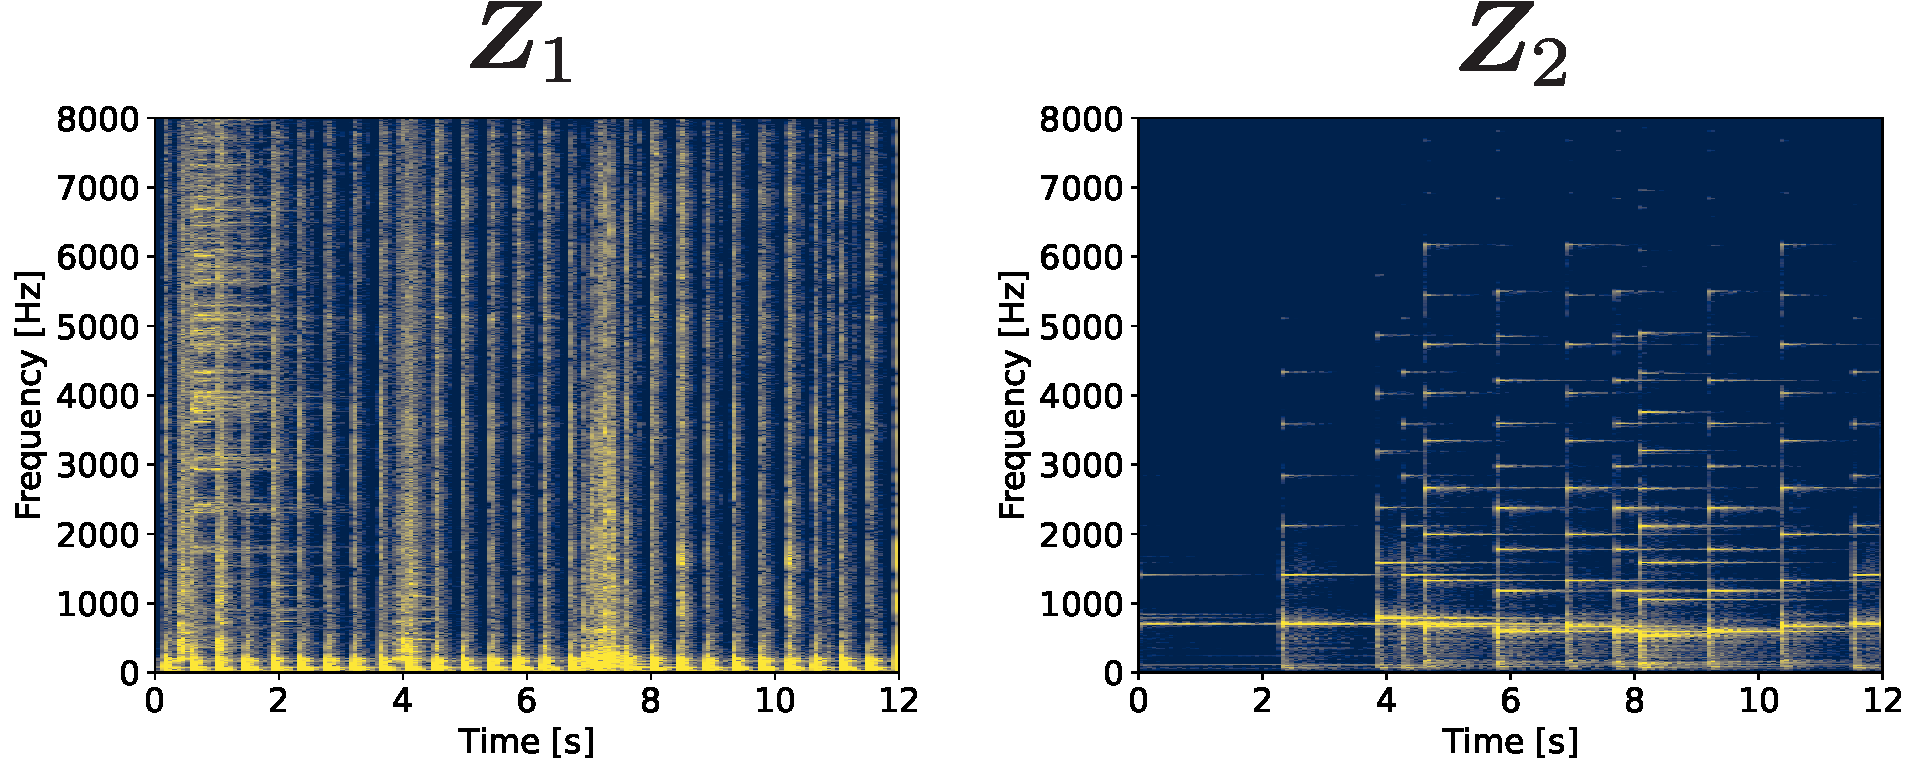
\includegraphics[width=0.95\columnwidth]{figures/Drum_init_spec.pdf}
  \end{center}
  \vspace{-8pt}
\caption{Uncertainty in ICA. ICA cannot determine order and scales of estimated signals.}
\label{fig:drum}
\end{figure}
%%%%%%%%%%%%%%%%%%%%%%%%%%%%
%----------------------------------------------

実際の音響信号に対して提案手法がどの程度適用できるかを調べるために,Table~\ref{table:wav}に示すようにSiSEC2011~\cite{Sisec}の英語の音声信号(男性1名及び女性1名)2種類と楽器音(ピアノとドラム)2種類を使用した.
音声信号のスペクトログラムをFig.~\ref{fig:audio},楽器音のスペクトログラムをFig.~\ref{fig:drum}に示す.
音響信号に対するSTFTは,fftサイズ2048~ms,シフトサイズ1024~msに設定した.音声信号と楽器音の分離に対しては,ブロックパーミュテーション問題を解くことを想定し,16行毎に周波数成分をシャッフルした場合の実験を行った.
最適化法やハイパーパラメータについては,\ref{sec:ex_condition_matrix}項の条件と同じである.
%----------------------------------------------
\section{実験結果}
\label{sec:ex_res}
%----------------------------------------------
%----------------------------------------------
\subsection{人工データに対する実験結果}
\label{sec:ex_res_artificial}
%----------------------------------------------


%%%%%%%%%%%%%%%%%%%%%%%%%%%%
\begin{figure*}[!t]
    \centering
    \subfloat[Percentage of correct answers for training and validation data.]{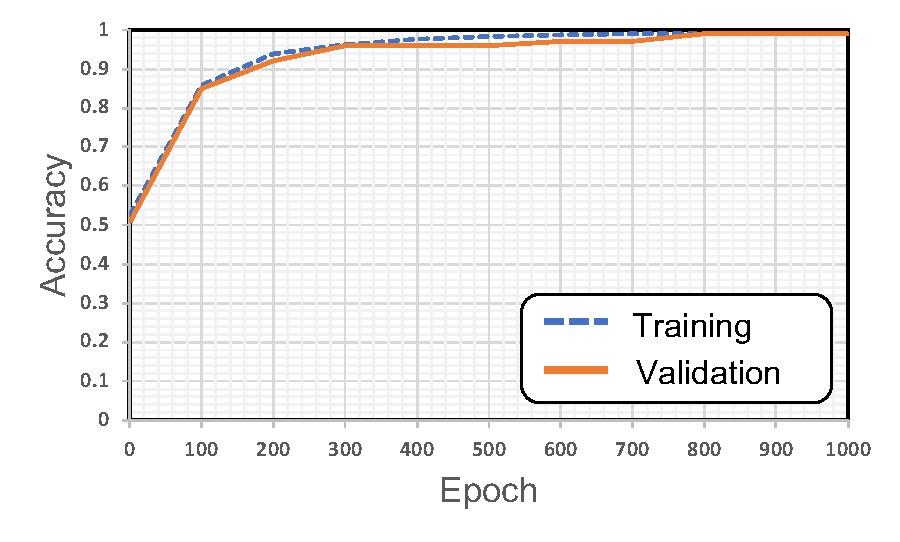
\includegraphics[clip, width=4.5in]{figures/01mat_1block_graph.pdf}
    \label{fig:acc_01mat_1block}}
    \\
    \subfloat[Spectrogram of estimated signal and predictive separation signal.]{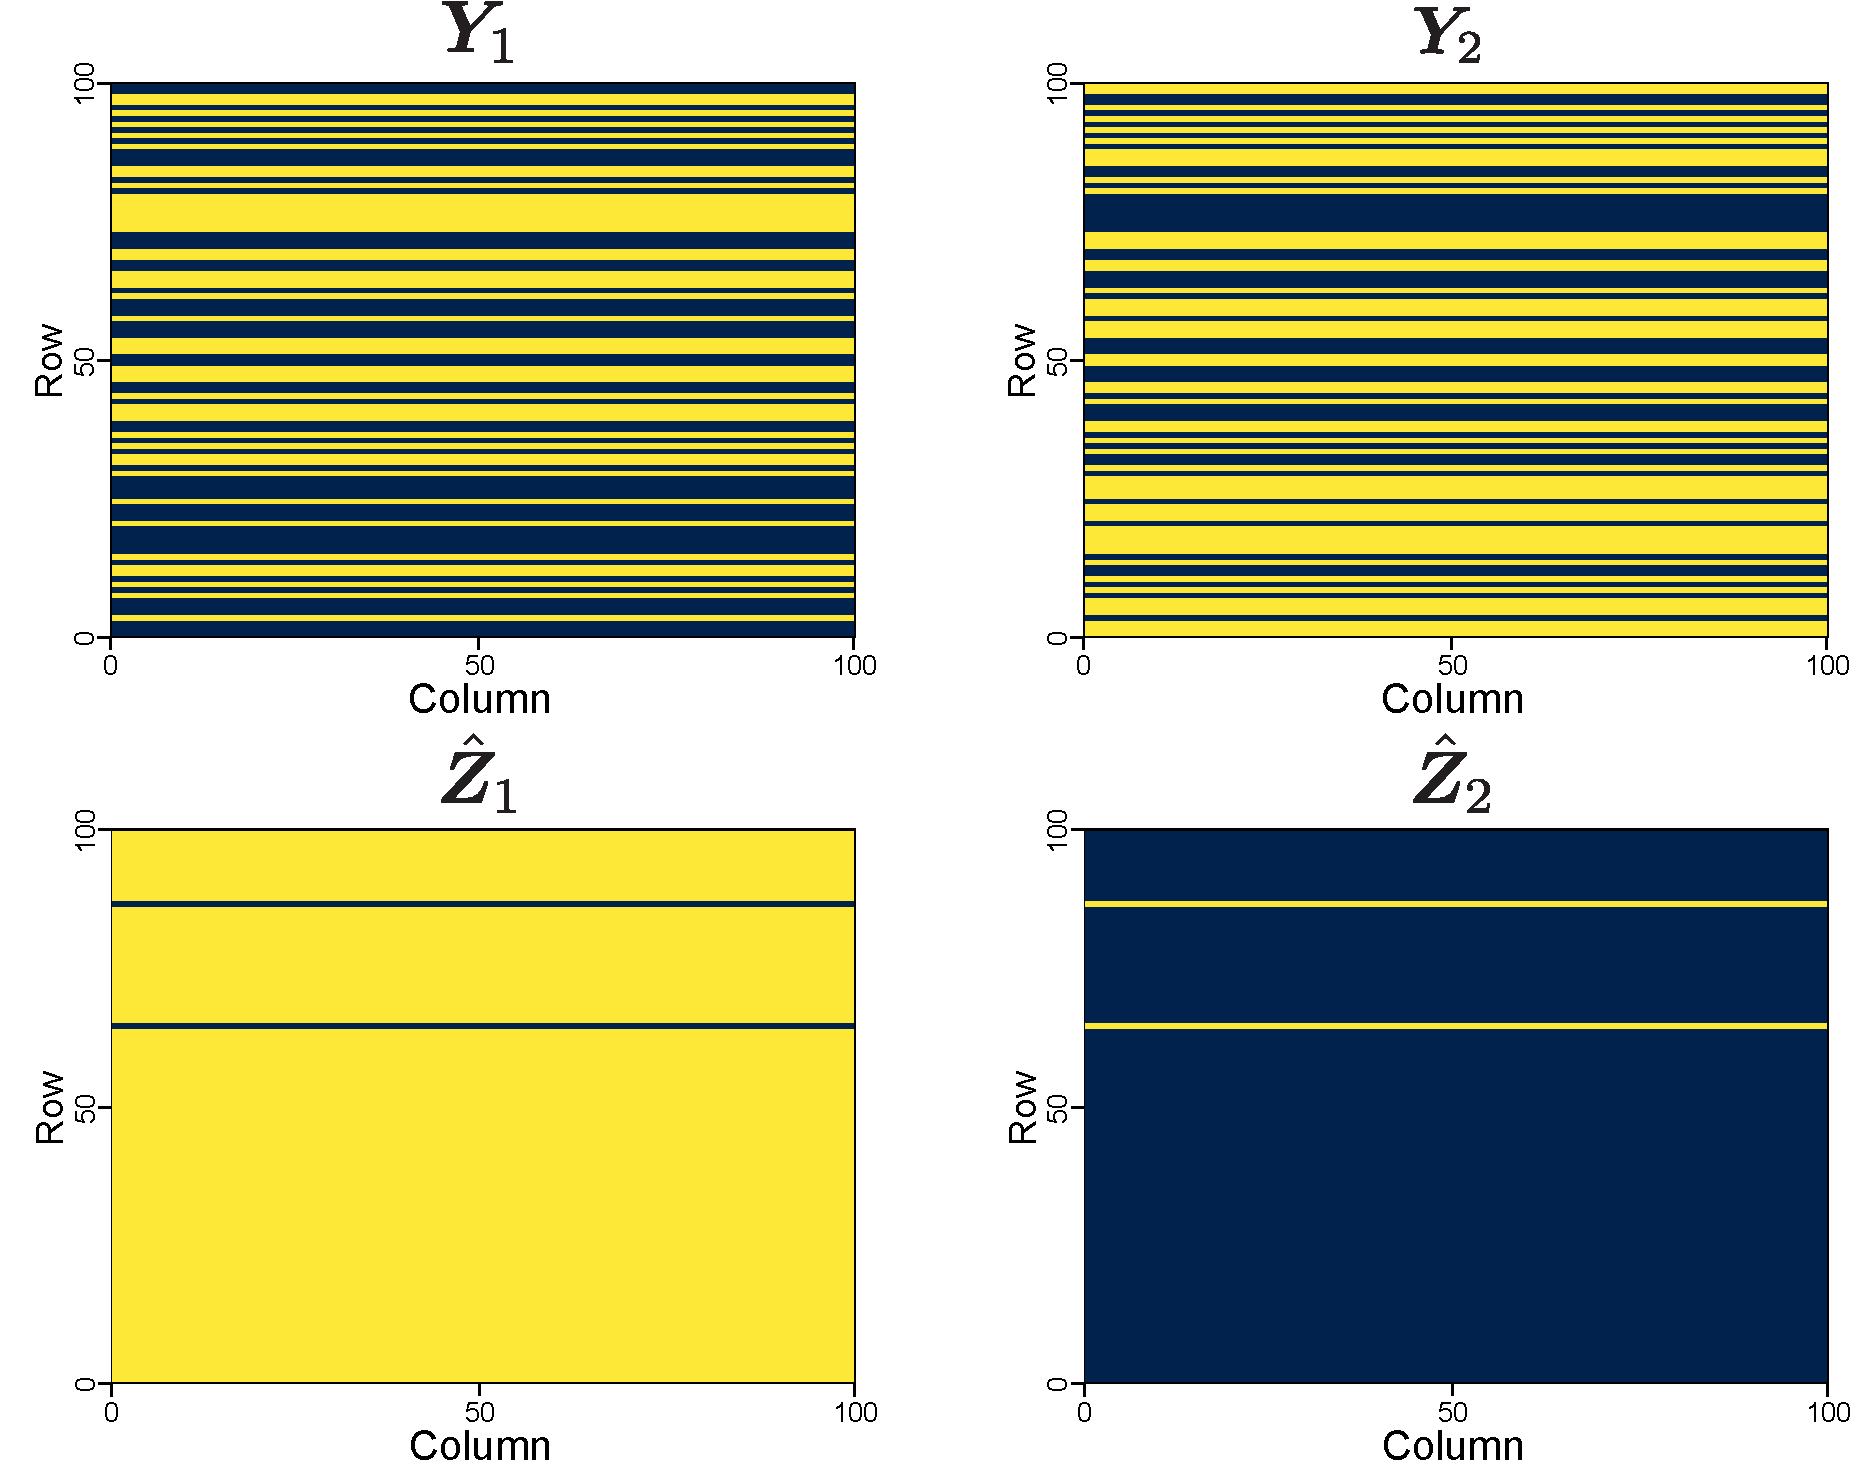
\includegraphics[clip, width=5.0in]{figures/01mat_1block.pdf}
    \label{fig:spec_01mat_1block}}  
    \caption{Experimental results using matrix of Fig~\ref{fig:01mat_spec} (shuffle the frequency per line).}
    \label{fig:01mat_1block}
\end{figure*}
%%%%%%%%%%%%%%%%%%%%%%%%%%%%

%%%%%%%%%%%%%%%%%%%%%%%%%%%%
\begin{figure*}[!t]
    \centering
    \subfloat[Percentage of correct answers for training and validation data.]{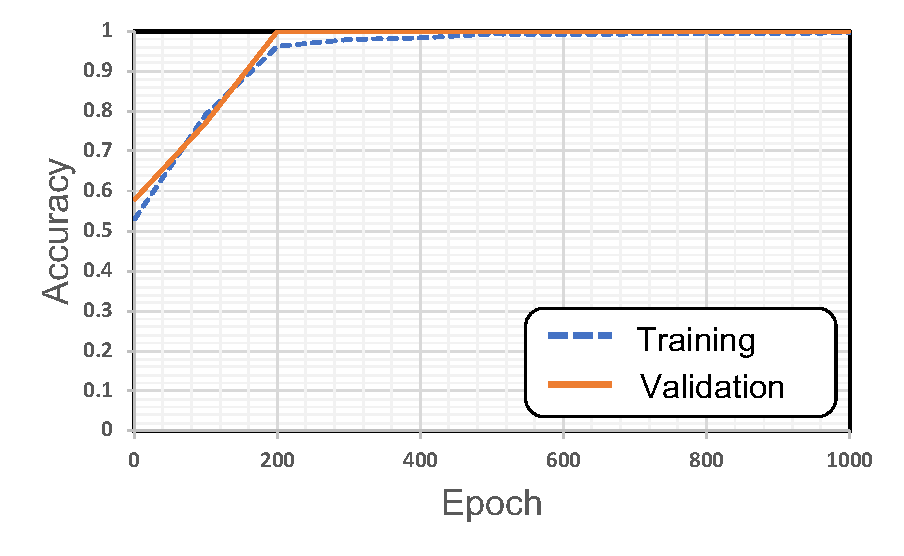
\includegraphics[clip, width=4.5in]{figures/graph_25stripe_1block.pdf}
    \label{fig:acc_25mat_1block}}
    \\
    \subfloat[Spectrogram of estimated signal and predictive separation signal.]{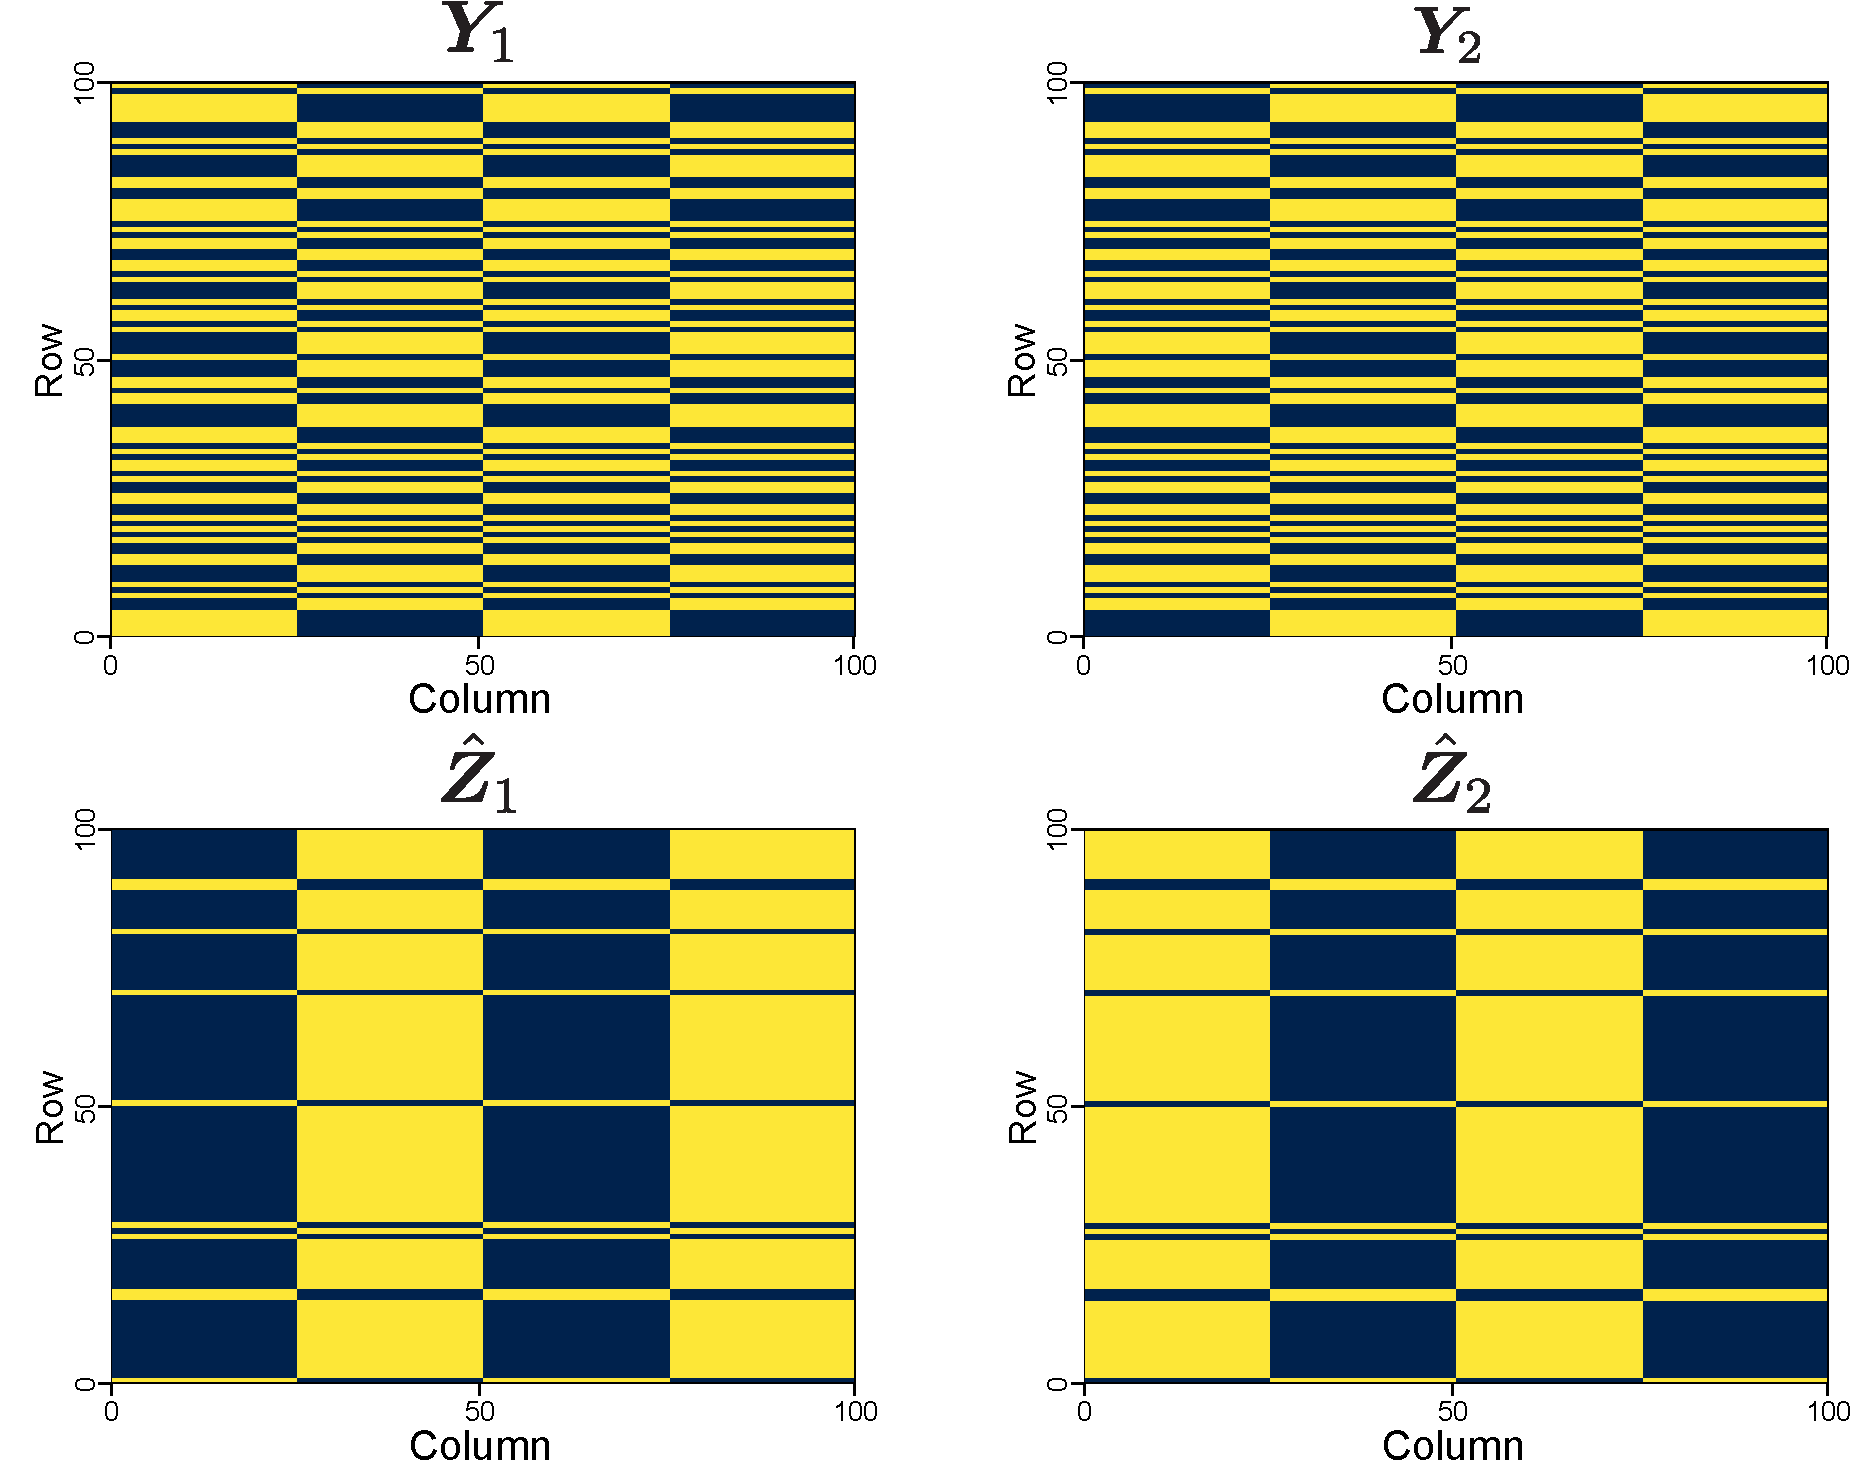
\includegraphics[clip, width=5.0in]{figures/25stripe_1block.pdf}
    \label{fig:spec_25mat_1block}}  
    \caption{Experimental results using the matrix of Fig~\ref{fig:25stripe_spec} (shuffle the frequency per row).}
    \label{fig:25mat_1block}
\end{figure*}
%%%%%%%%%%%%%%%%%%%%%%%%%%%%

%%%%%%%%%%%%%%%%%%%%%%%%%%%%
\begin{figure*}[!t]
    \centering
    \subfloat[Percentage of correct answers for training and validation data.]{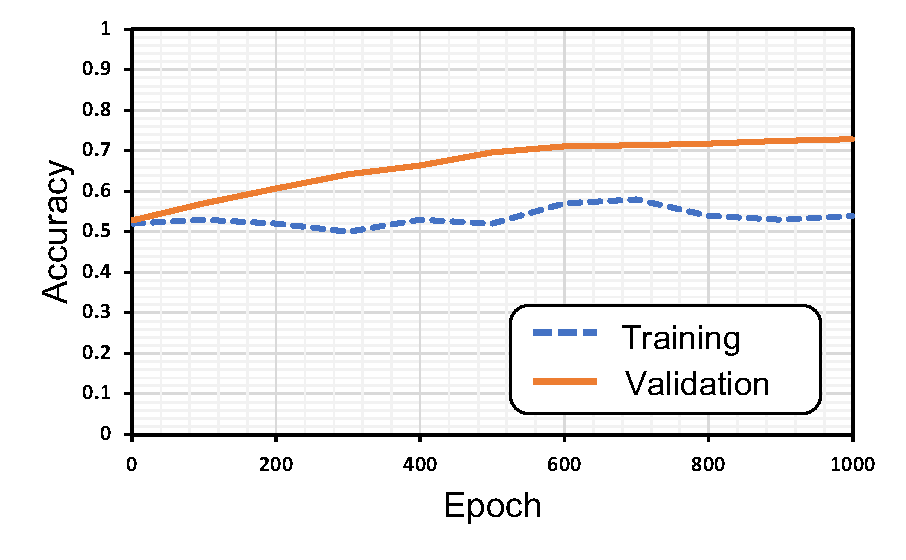
\includegraphics[clip, width=4.5in]{figures/graph/graph_stripe_1block.pdf}
    \label{fig:acc_stripe_1block}}
    \\
    \subfloat[Spectrogram of estimated signal and predictive separation signal.]{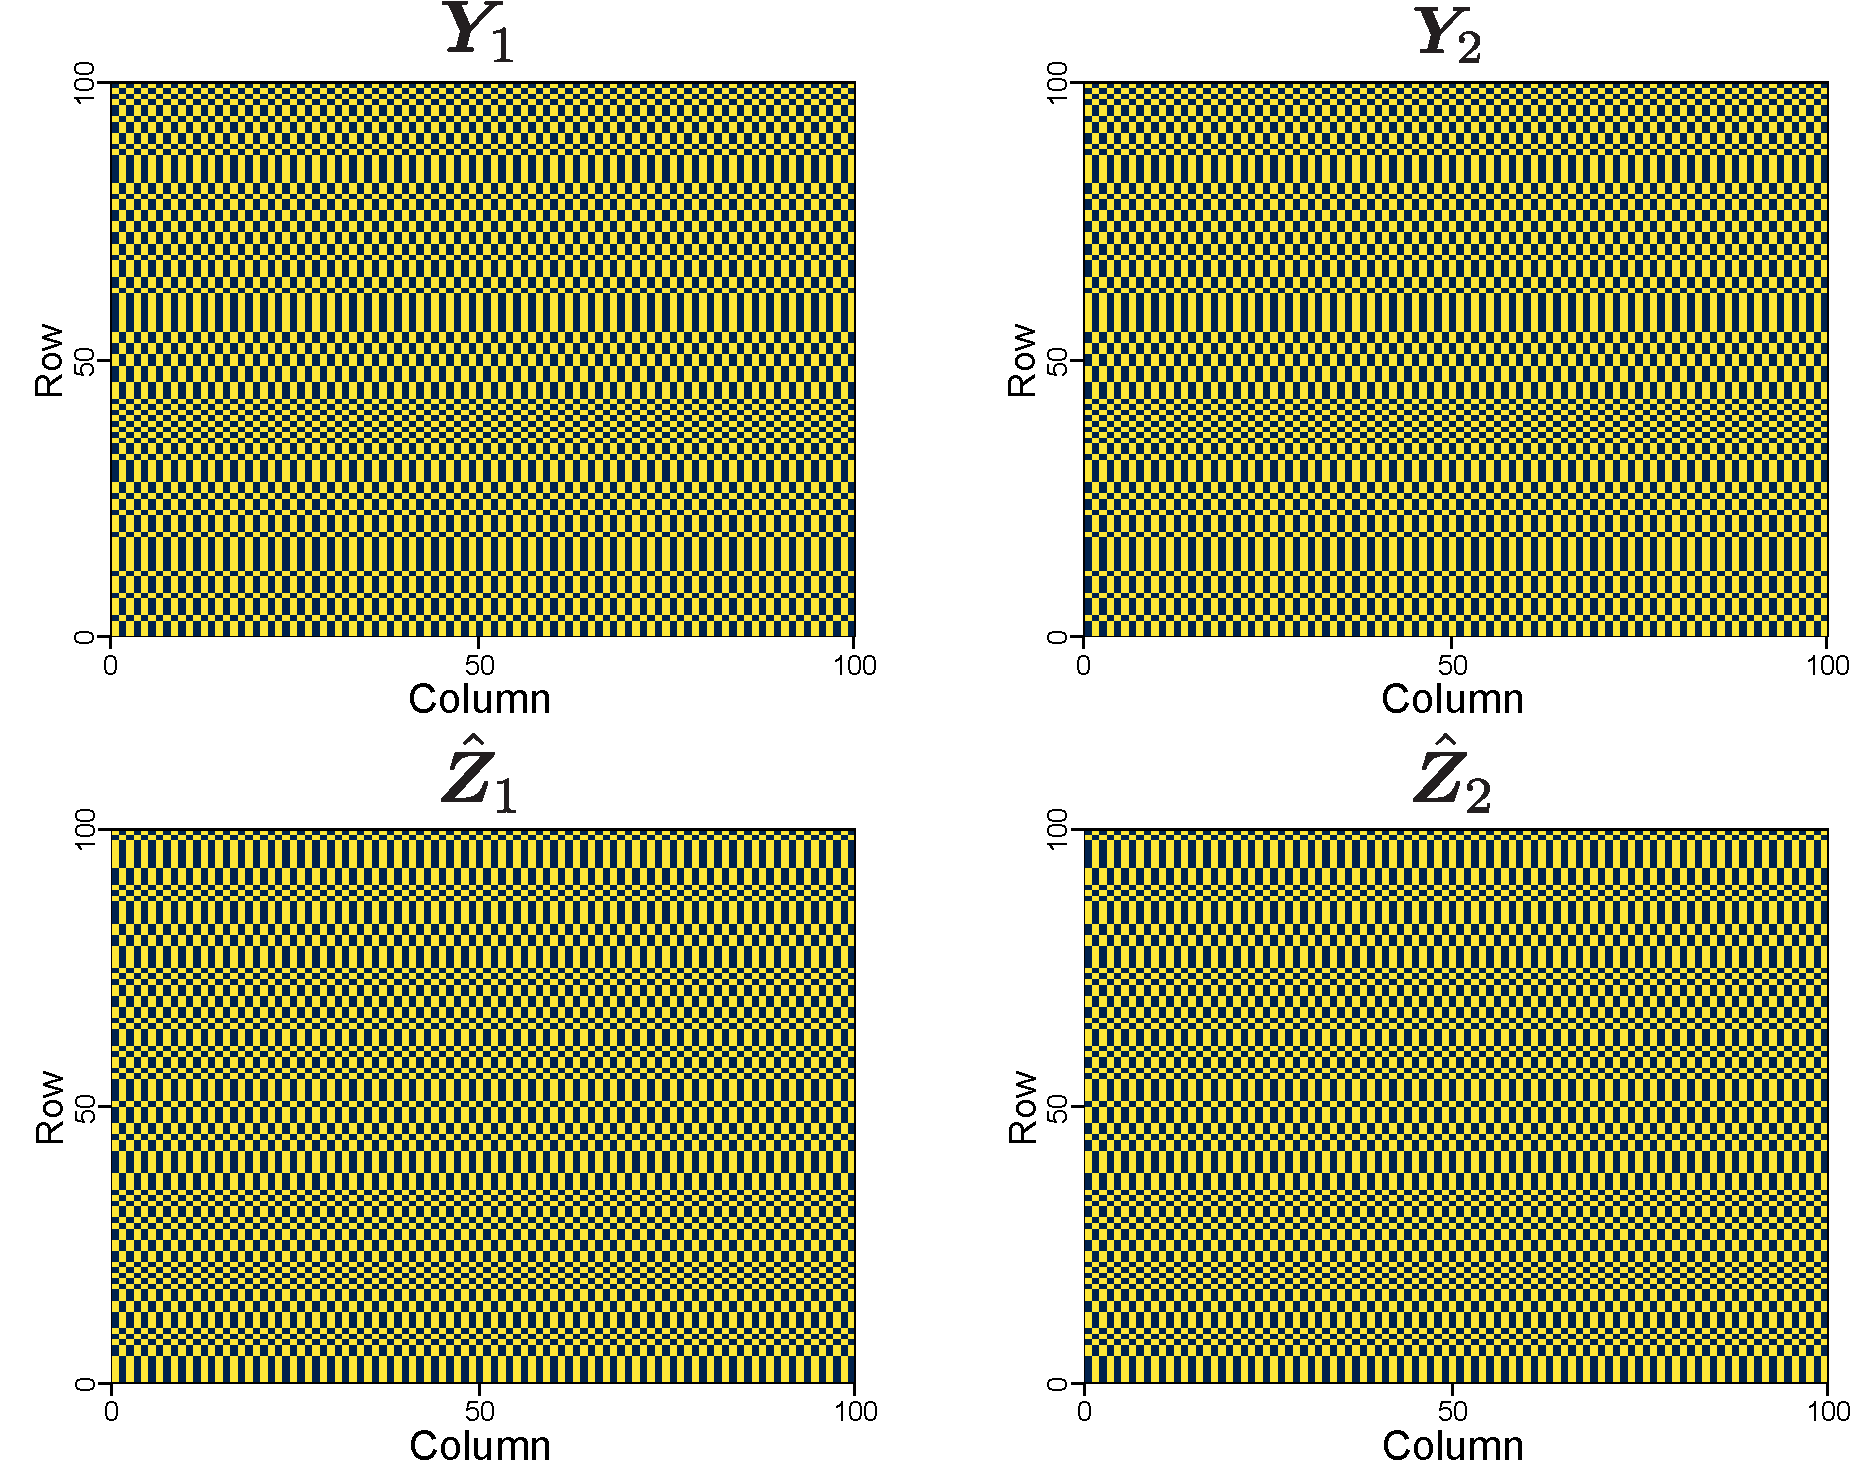
\includegraphics[clip, width=5.0in]{figures/stripe_1block.pdf}
    \label{fig:spec_stripe_1block}}  
    \caption{Experimental results using the matrix of Fig~\ref{fig:stripe_spec} (shuffle the frequency per row).}
    \label{fig:stripe_1block}
\end{figure*}
%%%%%%%%%%%%%%%%%%%%%%%%%%%%

%%%%%%%%%%%%%%%%%%%%%%%%%%%%
\begin{figure*}[!t]
    \centering
    \subfloat[Percentage of correct answers for training and validation data.]{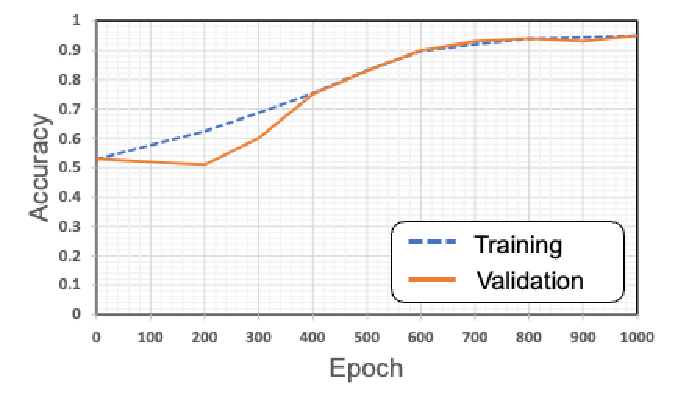
\includegraphics[clip, width=4.5in]{figures/graph_stripe_1block95ratio.pdf}
    \label{fig:acc_stripe_95ratio_1block}}
    \\
    \subfloat[Spectrogram of estimated signal and predictive separation signal.]{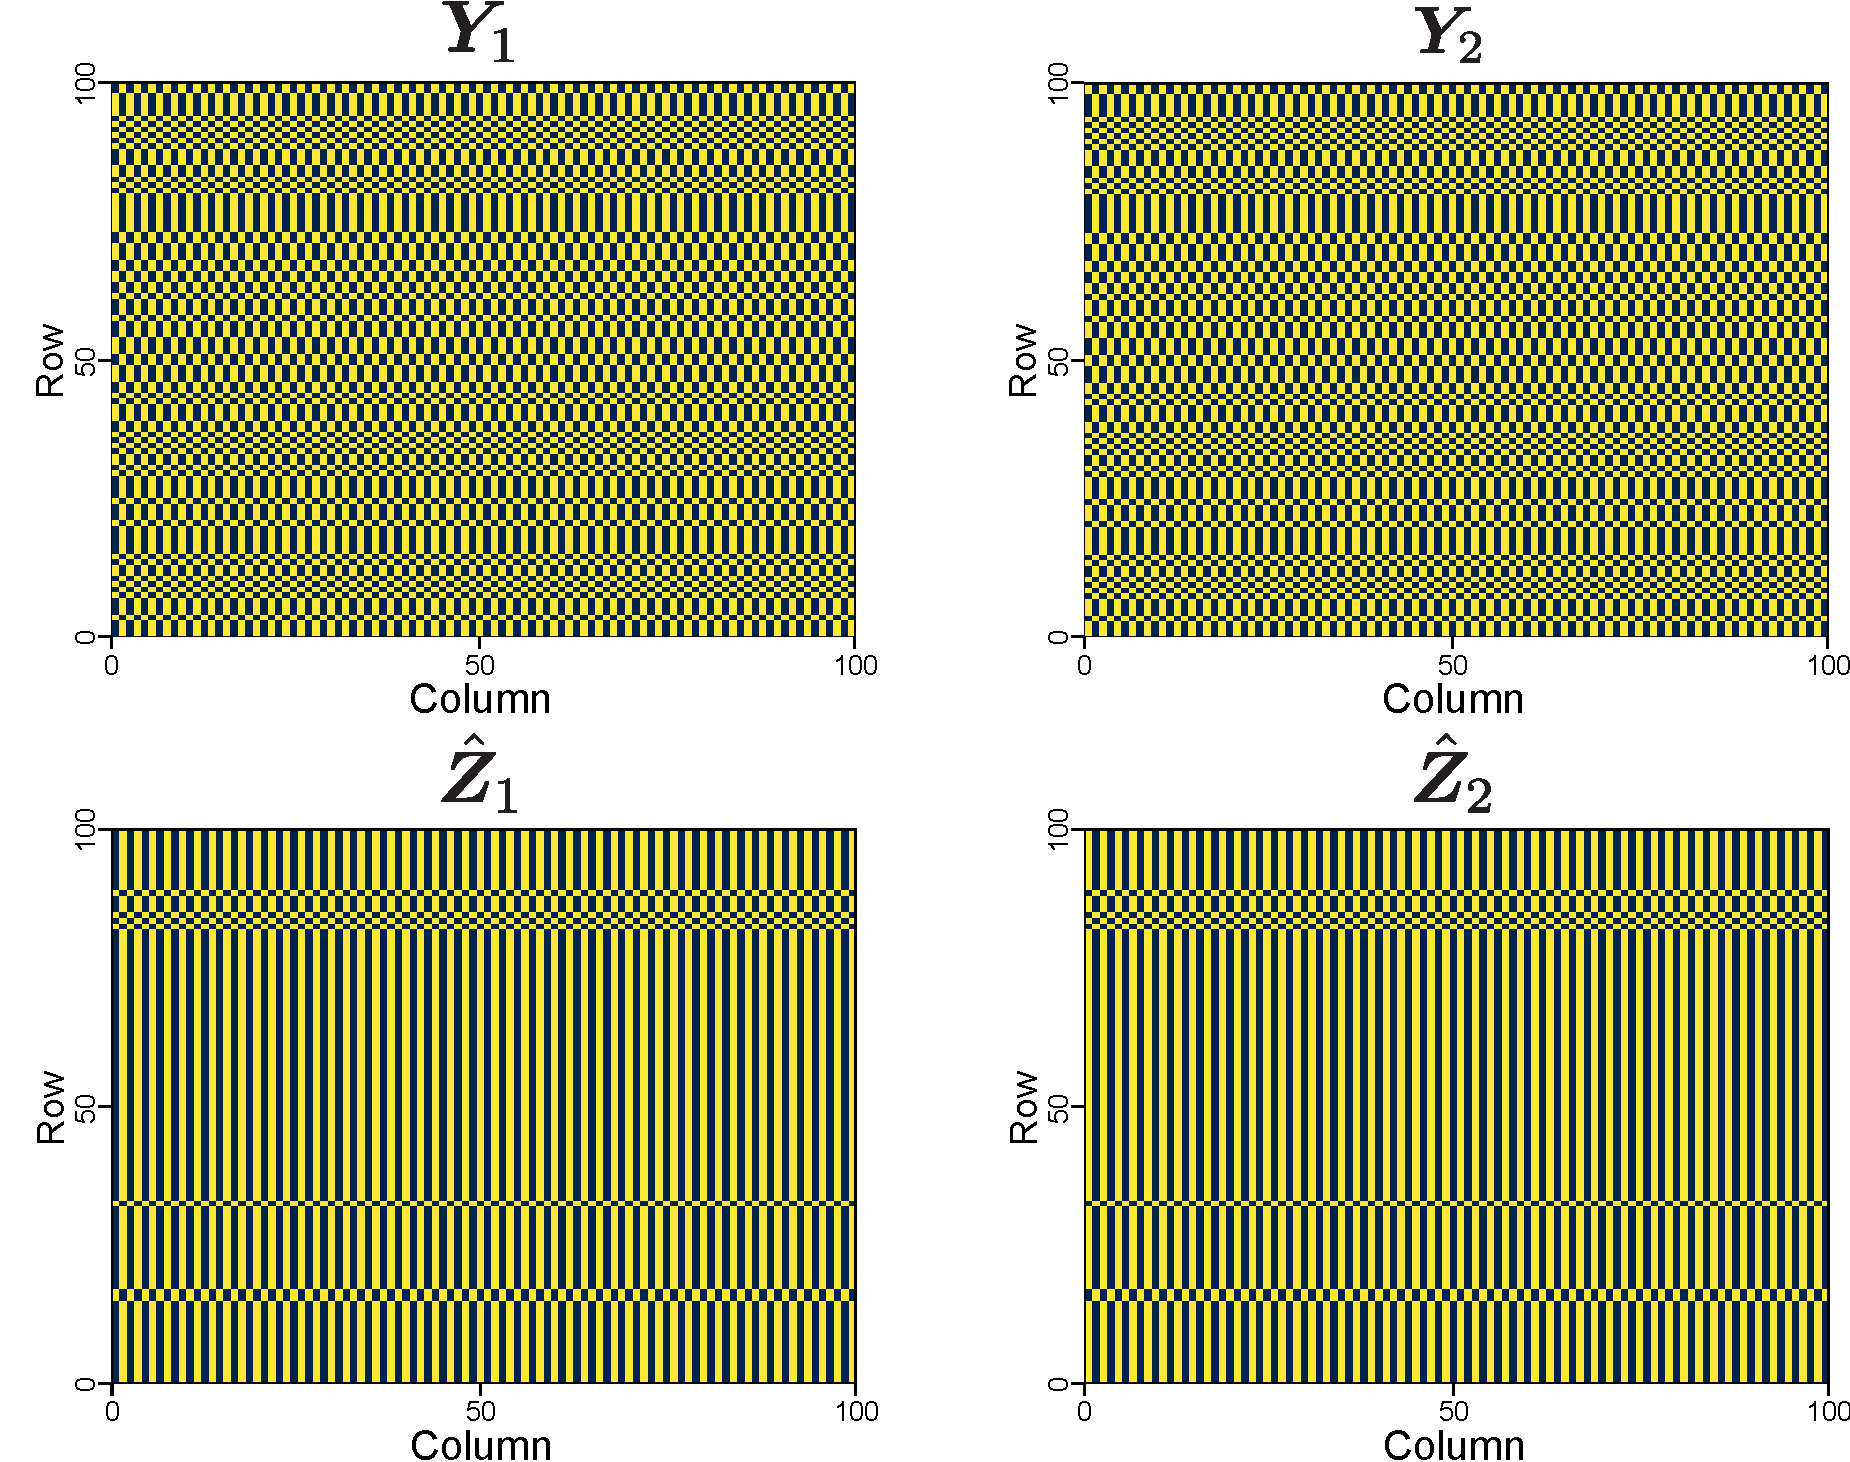
\includegraphics[clip, width=5.0in]{figures/stripe95ratio_1block_spec.pdf}
    \label{fig:spec_stripe_95ratio_1block}}  
    \caption{Experimental results using the matrix of Fig~\ref{fig:stripe_spec} (shuffle every row 95\% of the time, and every two rows 5\% of the time).}
    \label{fig:stripe_95ratio_1block}
\end{figure*}
%%%%%%%%%%%%%%%%%%%%%%%%%%%%

%%%%%%%%%%%%%%%%%%%%%%%%%%%%
\begin{figure*}[!t]
    \centering
    \subfloat[Percentage of correct answers for training and validation data.]{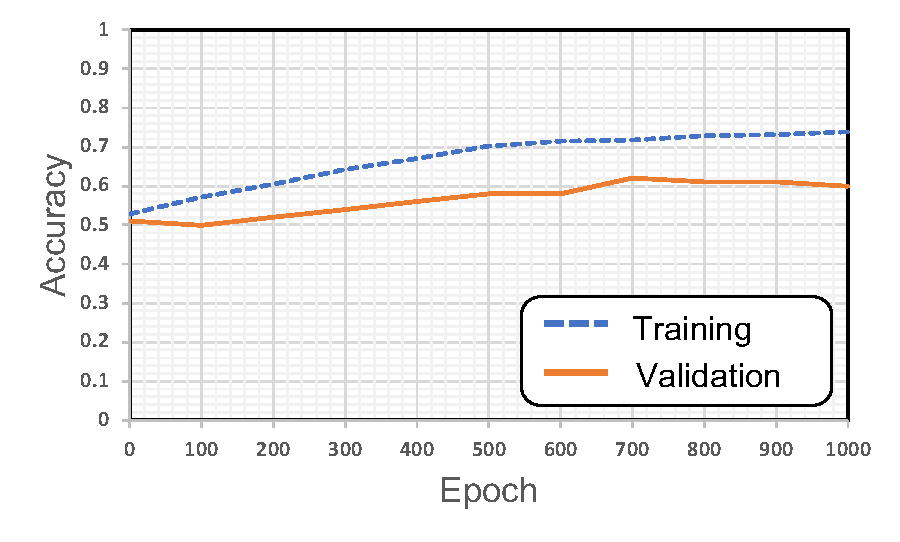
\includegraphics[clip, width=4.5in]{figures/graph/stripe_1block99ratio.pdf}
    \label{fig:acc_stripe_99ratio_1block}}
    \\
    \subfloat[Spectrogram of estimated signal and predictive separation signal.]{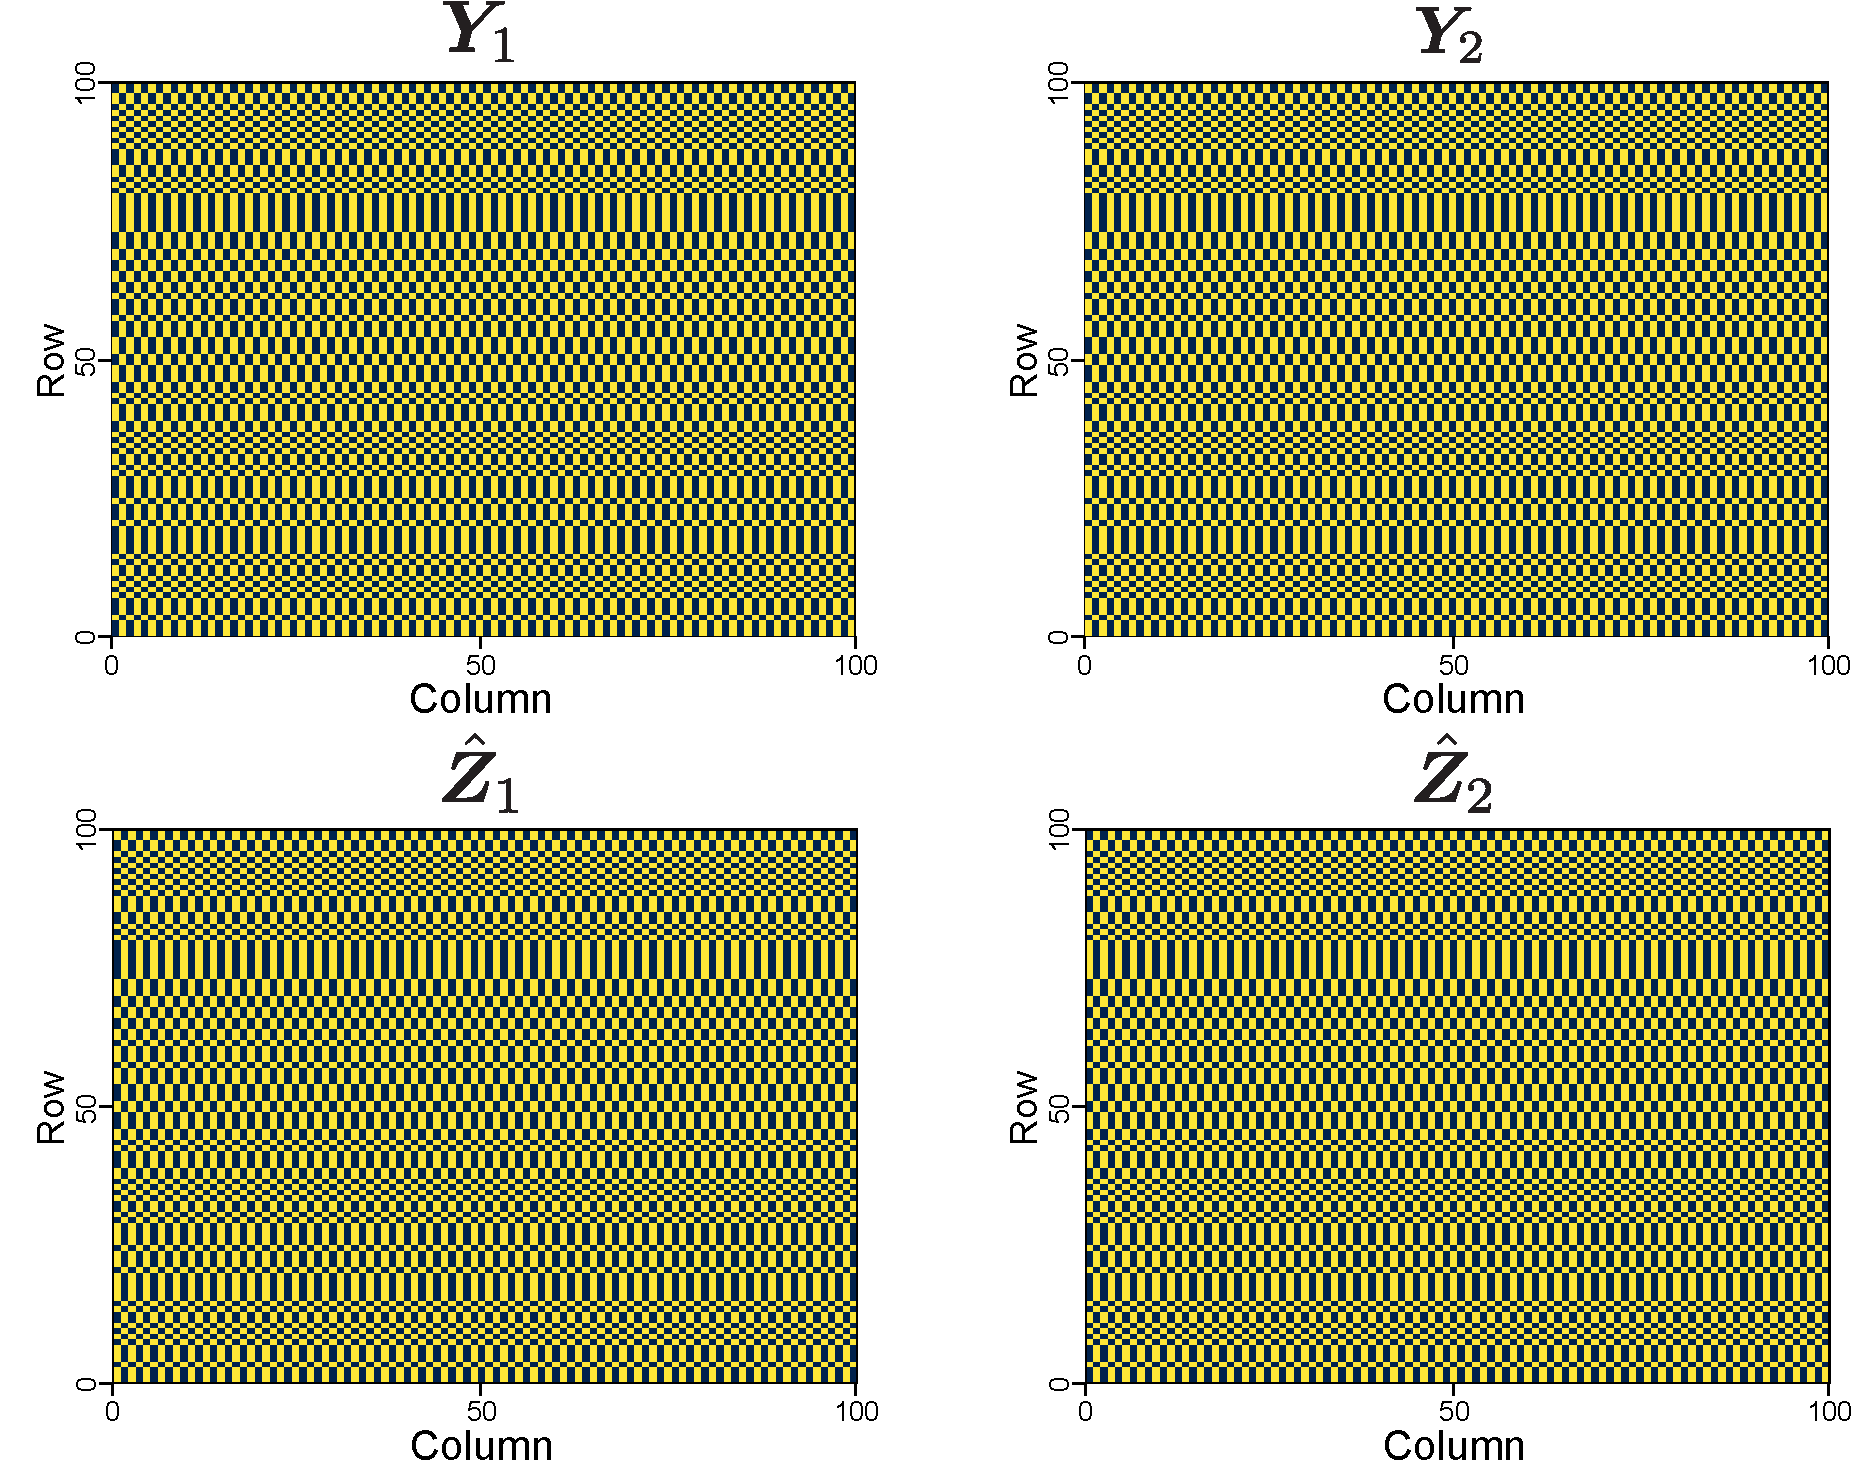
\includegraphics[clip, width=5.0in]{figures/stripe99ratio_1block_spec.pdf}
    \label{fig:spec_stripe_99ratio_1block}}  
    \caption{Experimental results using the matrix of Fig~\ref{fig:stripe_spec} (shuffle every row 99\% of the time, and every two rows 5\% of the time).}
    \label{fig:stripe_99ratio_1block}
\end{figure*}
%%%%%%%%%%%%%%%%%%%%%%%%%%%%

Fig.~\ref{fig:01mat_1block}--\ref{fig:stripe_1block}には,全ての成分が0と1の行列,25列毎に0と1の値が入れ替わる行列,1列毎に0と1の値が入れ替わる行列の周波数成分に対して各周波数毎にシャッフルを行った時の結果を示す.
この結果から,各周波数成分毎にシャッフルした場合,Fig.~\ref{fig:01mat_spec}やFig.~\ref{fig:25stripe_spec}に示すような,比較的簡易的な行列に対しては,それぞれ正答率が100\%に近い値となっている.
Fig.~\ref{fig:01mat_spec}とFig.~\ref{fig:25stripe_spec}の$\hat{\bm{Z}}_1$,$\hat{\bm{Z}}_2$は少しの間違いは含んでいるものの,おおよそ並び替えができていることが分かる.
しかし,Fig.~\ref{fig:stripe_spec}に示すような,1列毎に0と1の値が入れ替わる行列に対して各周波数成分毎にシャッフルを行った場合は,Fig.~\ref{fig:stripe_1block}に示すように正答率が54\%程度となった.
$\hat{\bm{Z}}_1$,$\hat{\bm{Z}}_2$を見ても並び替えができていないことが分かる.
即ち,提案手法において各行毎にシャッフルを行なった行列に対してはパーミュテーション問題を解決することが難しいが,ブロック単位でのパーミュテーション問題は容易に解けると言える.
Fig.~\ref{fig:stripe_95ratio_1block}及びFig.~\ref{fig:stripe_99ratio_1block}は,5\%の割合で2行毎にシャッフルしそれ以外は1行毎にシャッフルした行列と,
1\%の割合で2行毎シャッフルしそれ以外は1行毎にシャッフルした行列を用いて実験を行った結果を示す.5\%の割合で2行毎にシャッフルしそれ以外は1行毎にシャッフルした場合の正答率は93\%程度となったが,
1\%の割合で2行毎シャッフルしそれ以外は1行毎にシャッフルした場合の正答率は60\%程度となった.
このことより,DNNは少しでもブロック単位でシャッフルが行われていると学習が容易となることが分かる.

%%%%%%%%%%%%%%%%%%%%%%%%%%%%
\begin{figure*}[!t]
  \centering
  \subfloat[Percentage of correct answers for training and validation data.]{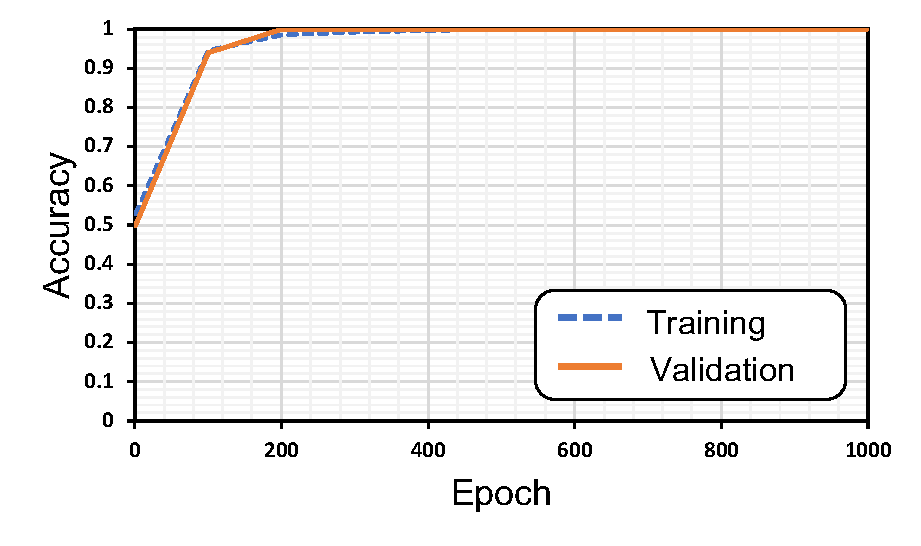
\includegraphics[clip, width=4.5in]{figures/graph/01mat_2block.pdf}
  \label{fig:acc_01mat_2block}}
  \\
  \subfloat[Spectrogram of estimated signal and predictive separation signal.]{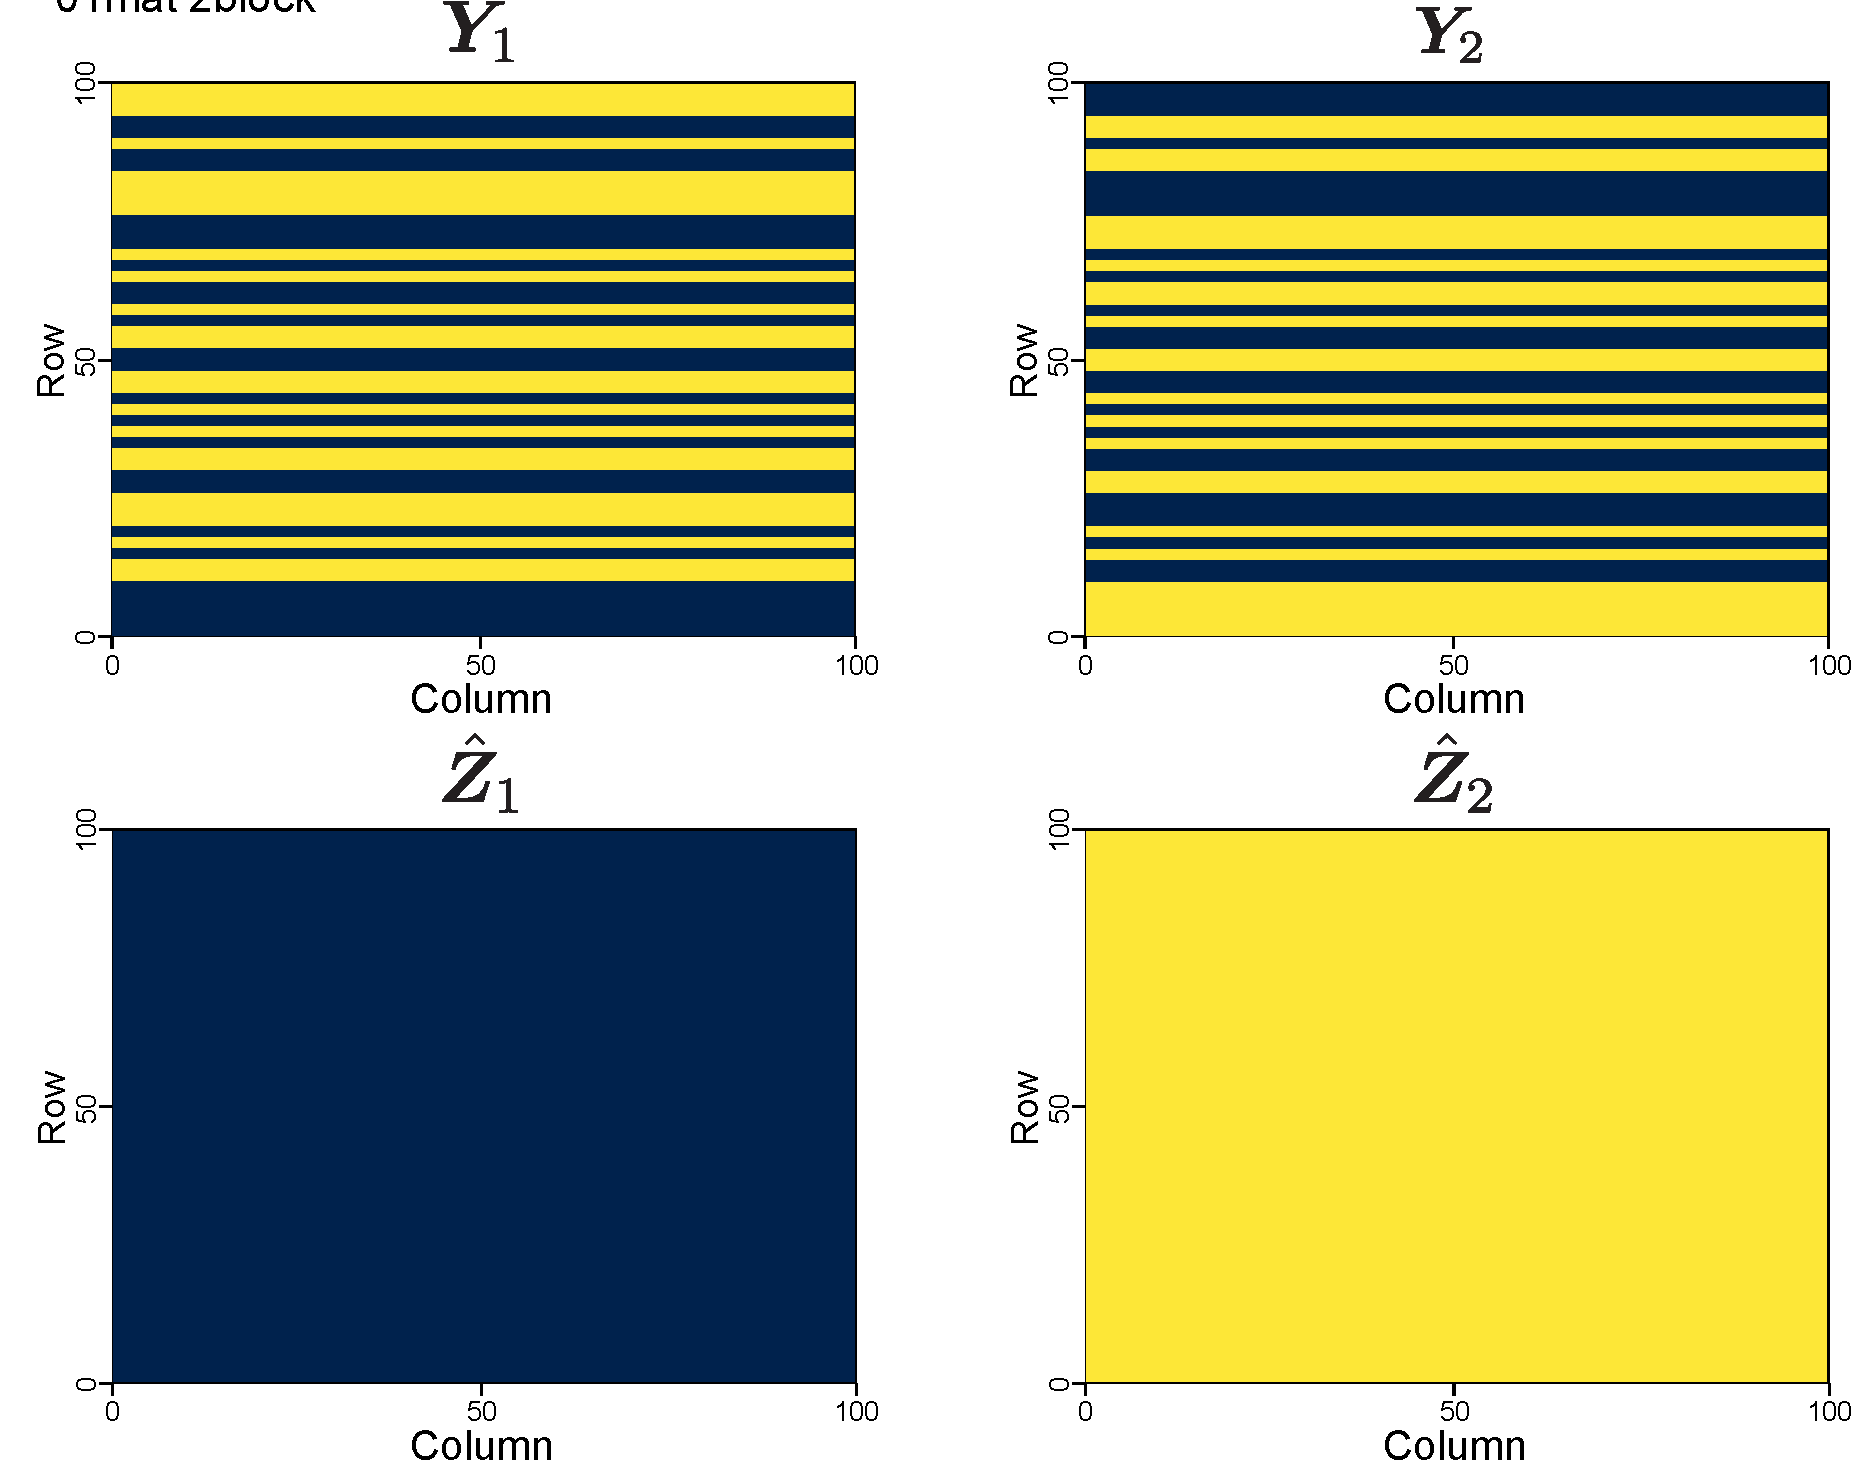
\includegraphics[clip, width=5.0in]{figures/01mat_2block.pdf}
  \vspace{-8pt}
  \label{fig:spec_01mat_2block}}
  \caption{Experimental results using the matrix of Fig~\ref{fig:01mat_spec} (shuffle the frequency every 2 rows).}
  \label{fig:01mat_2block}
\end{figure*}
%%%%%%%%%%%%%%%%%%%%%%%%%%%%

%%%%%%%%%%%%%%%%%%%%%%%%%%%%
\begin{figure*}[!t]
  \centering
  \subfloat[Percentage of correct answers for training and validation data.]{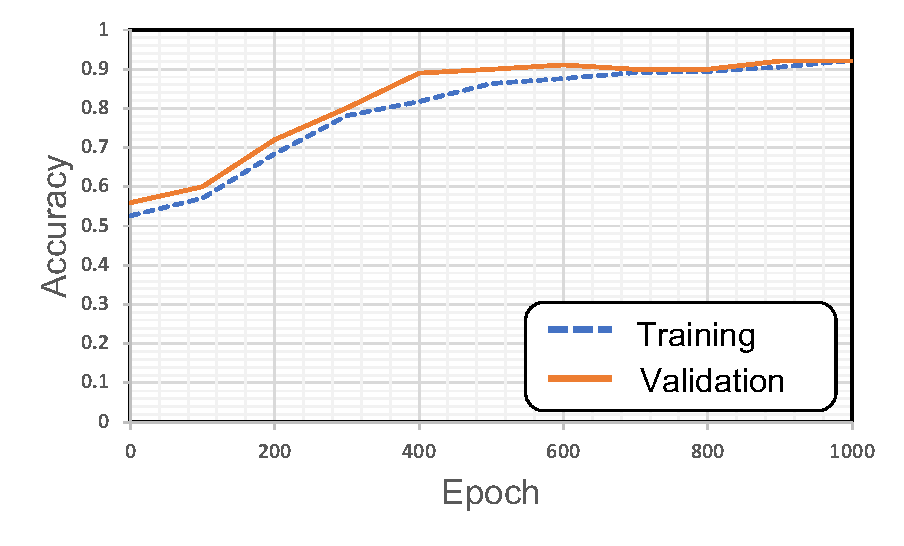
\includegraphics[clip, width=4.5in]{figures/graph/25stripe_2block.pdf}
  \label{fig:acc_25stripe_2block}}
  \\
  \subfloat[Spectrogram of estimated signal and predictive separation signal.]{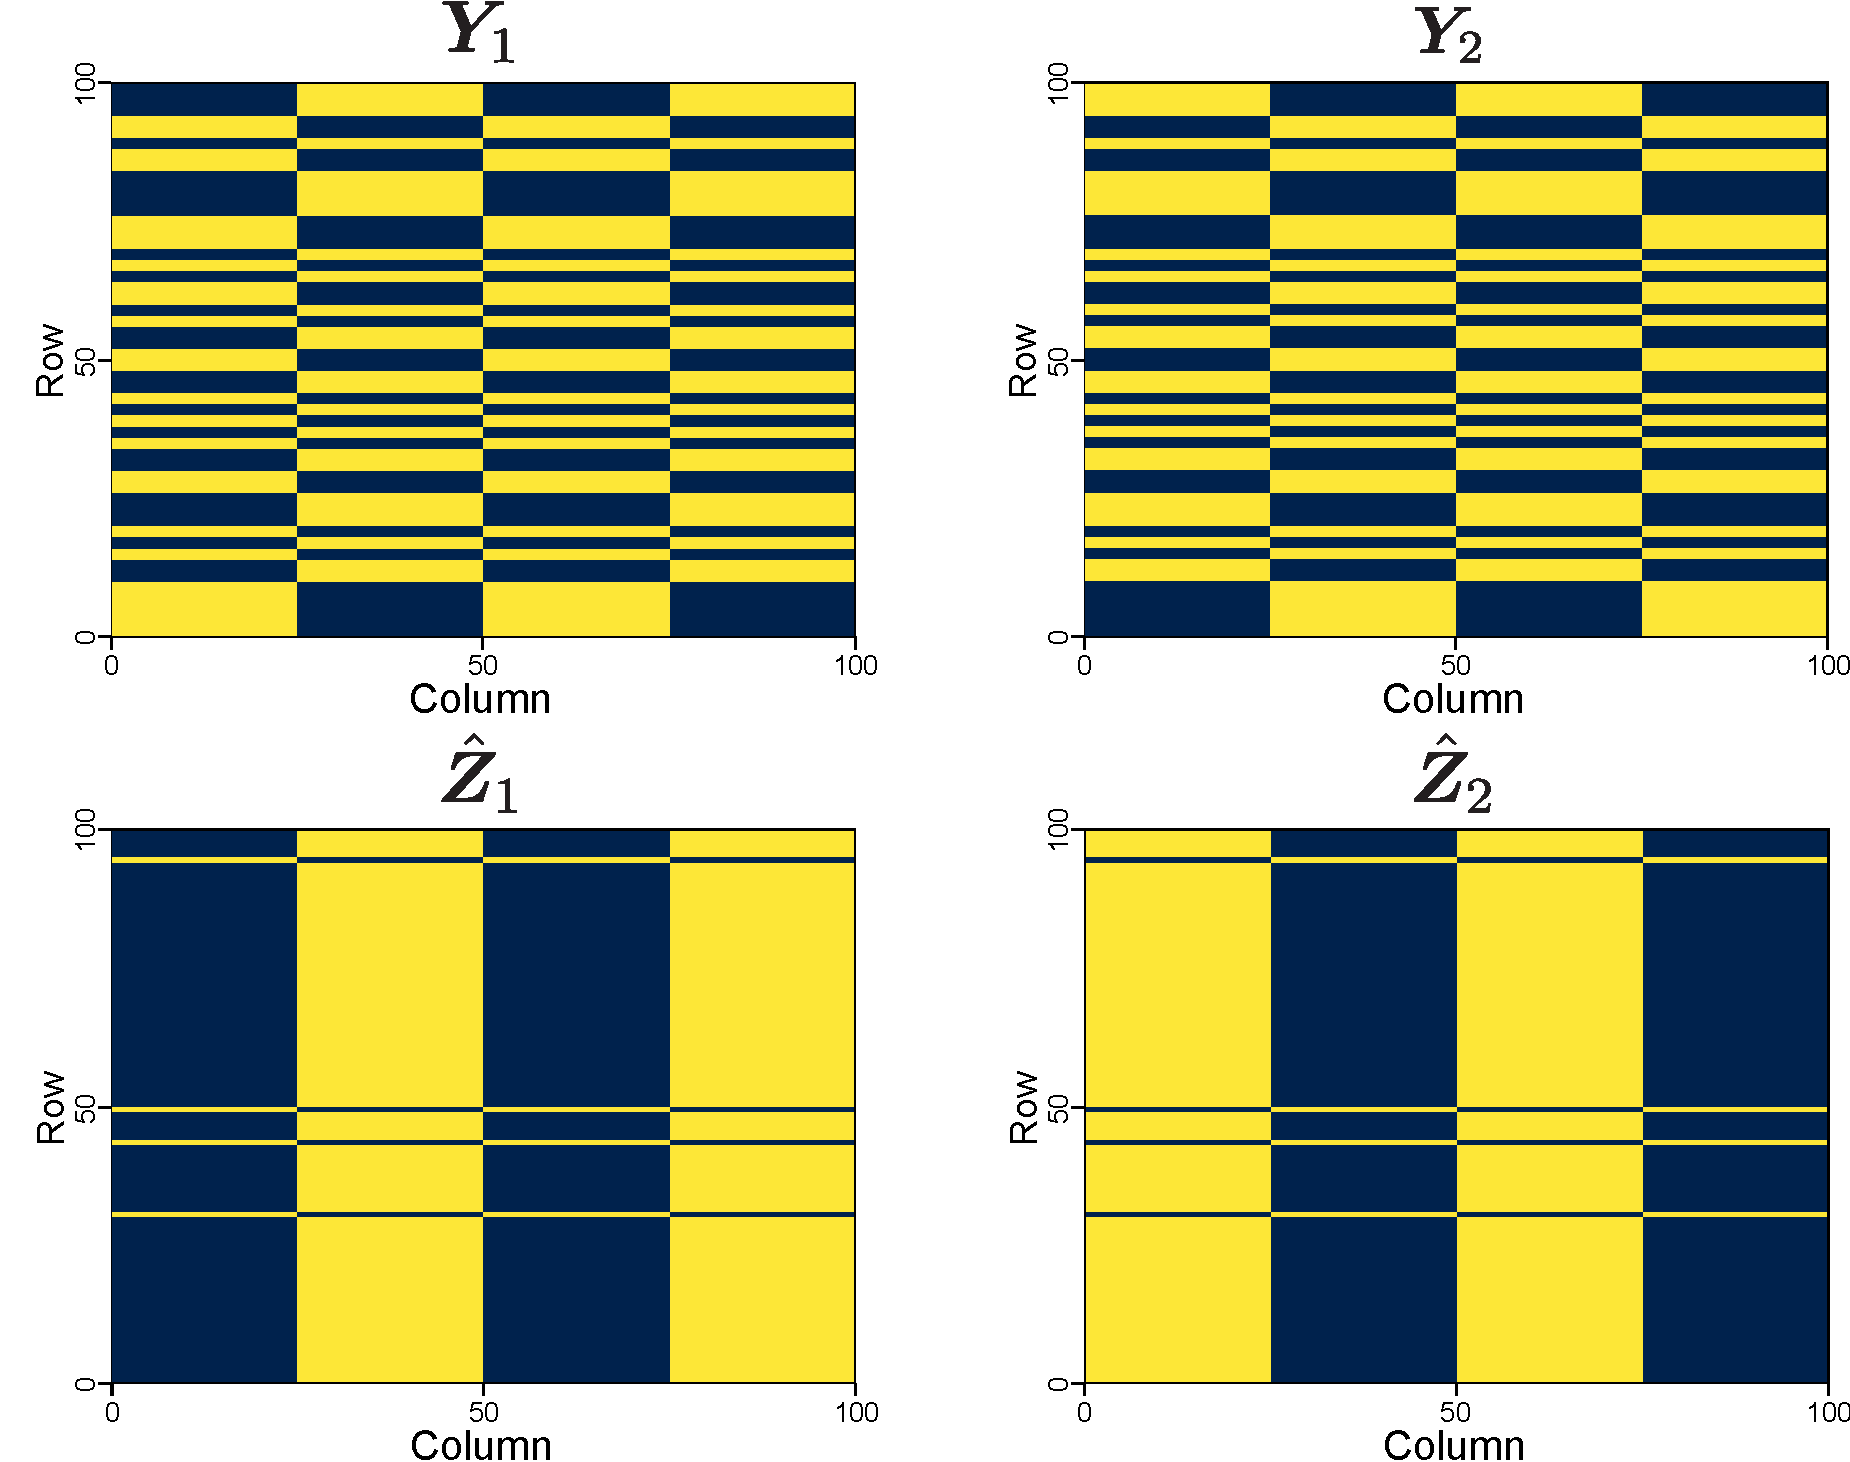
\includegraphics[clip, width=5.0in]{figures/25stripe_2block.pdf}
  \vspace{-8pt}
  \label{fig:spec_25stripe_2block}}
  \caption{Experimental results using the matrix of Fig~\ref{fig:25stripe_spec} (shuffle the frequency every 2 rows).}
  \label{fig:25stripe_2block}
\end{figure*}
%%%%%%%%%%%%%%%%%%%%%%%%%%%%

%%%%%%%%%%%%%%%%%%%%%%%%%%%%
\begin{figure*}[!t]
  \centering
  \subfloat[Percentage of correct answers for training and validation data.]{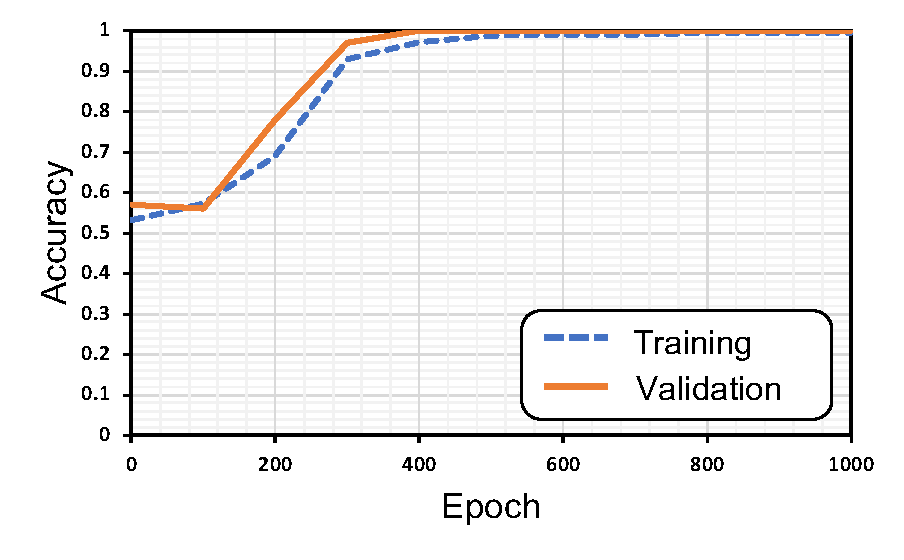
\includegraphics[clip, width=4.5in]{figures/graph/stripe_2block.pdf}
  \label{fig:acc_stripe_2block}}
  \\
  \subfloat[Spectrogram of estimated signal and predictive separation signal.]{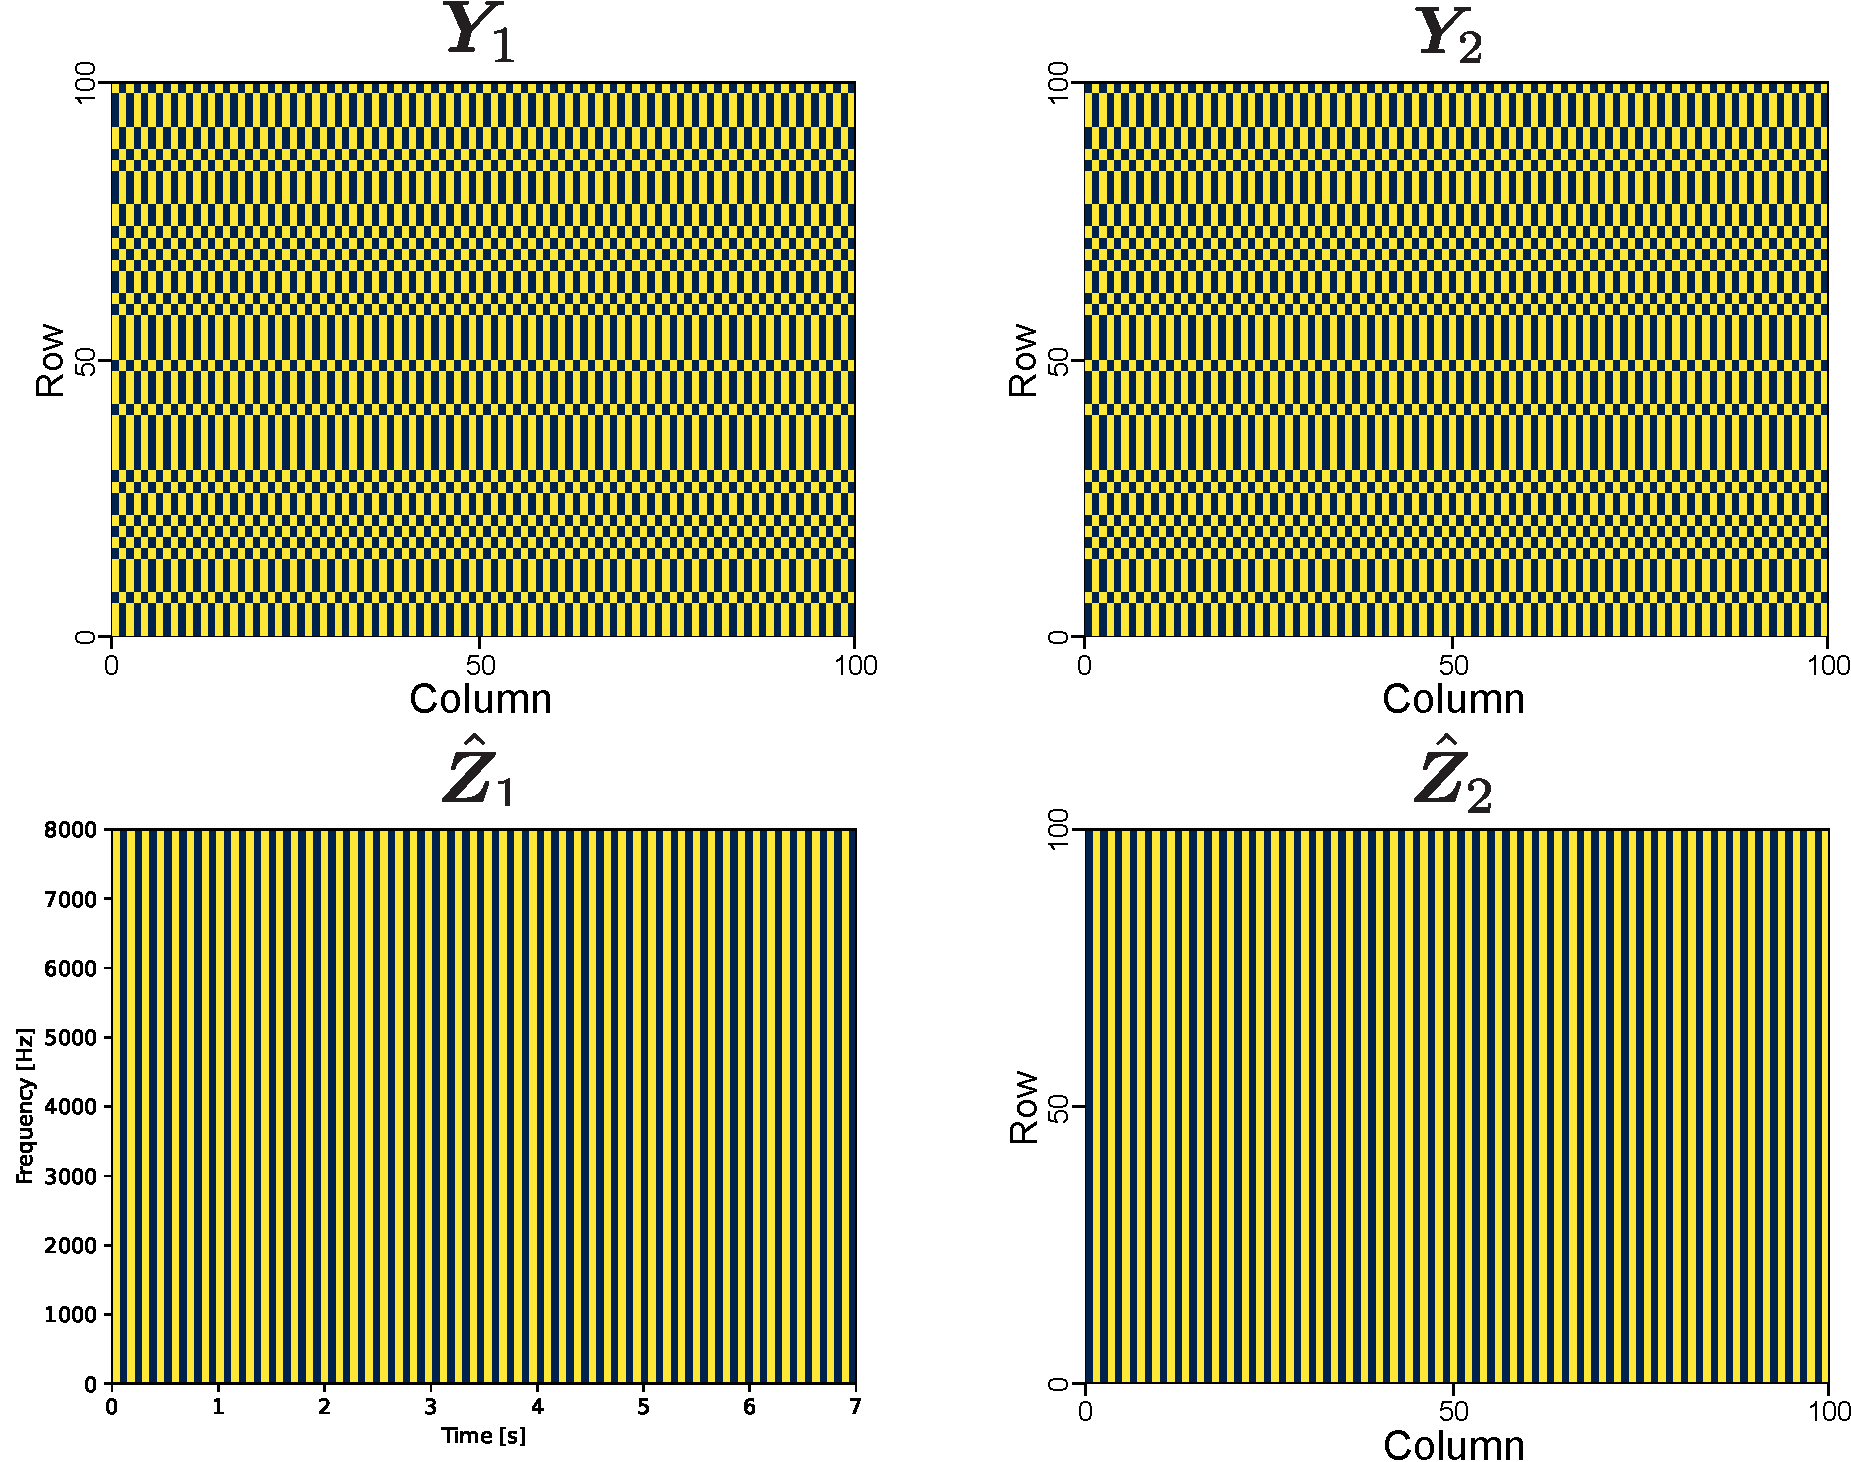
\includegraphics[clip, width=5.0in]{figures/stripe_2block.pdf}
  \vspace{-8pt}
  \label{fig:spec_stripe_2block}}
  \caption{Experimental results using the matrix of Fig~\ref{fig:stripe_spec} (shuffle the frequency every 2 rows).}
  \label{fig:stripe_2block}
\end{figure*}
%%%%%%%%%%%%%%%%%%%%%%%%%%%%

Fig.~\ref{fig:01mat_2block}--\ref{fig:stripe_2block}には,全ての成分が0と1の行列,
25列毎に0と1の値が入れ替わる行列,1列毎に0と1の値が入れ替わる行列の周波数成分に対して2行毎にシャッフルを行った時の結果を示す.
Fig.~\ref{fig:01mat_2block}--\ref{fig:stripe_2block}のどの実験結果も概ね推定分離信号$\hat{\bm{Z}}_1$,$\hat{\bm{Z}}_2$が正しい分離信号に近い値となっていることが分かる.
即ち,ある程度の塊毎に各周波数成分のシャッフルが行われているときはDNNは高精度で分離信号を予測することが可能であるといえる.
この他にも行列の周波数成分に対して4行毎と8行毎にシャッフルした時の実験を行なったが,結果が行列の周波数成分を2行毎に入れ替えた結果とほとんど同様であった.
従って,図として示すことは省略する.
\clearpage
%----------------------------------------------
\subsection{音声及び音楽信号に対する実験結果}
\label{sec:ex_res_artificial}
%----------------------------------------------

%%%%%%%%%%%%%%%%%%%%%%%%%%%%
\begin{figure*}[!t]
  \centering
  \subfloat[Percentage of correct answers for training and validation data.]{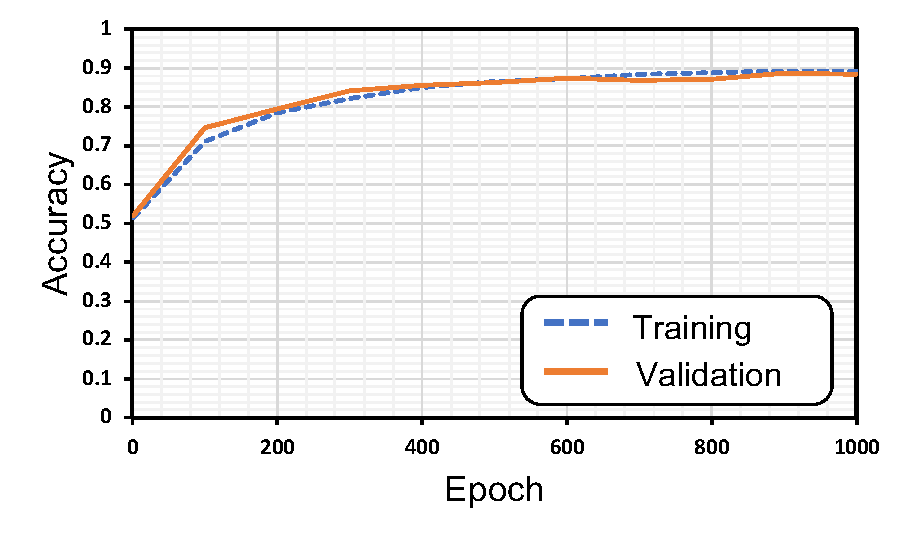
\includegraphics[clip, width=4.5in]{figures/graph/audio_16block.pdf}
  \label{fig:acc_audio_16block}}
  \\
  \subfloat[Spectrogram of estimated signal and predictive separation signal.]{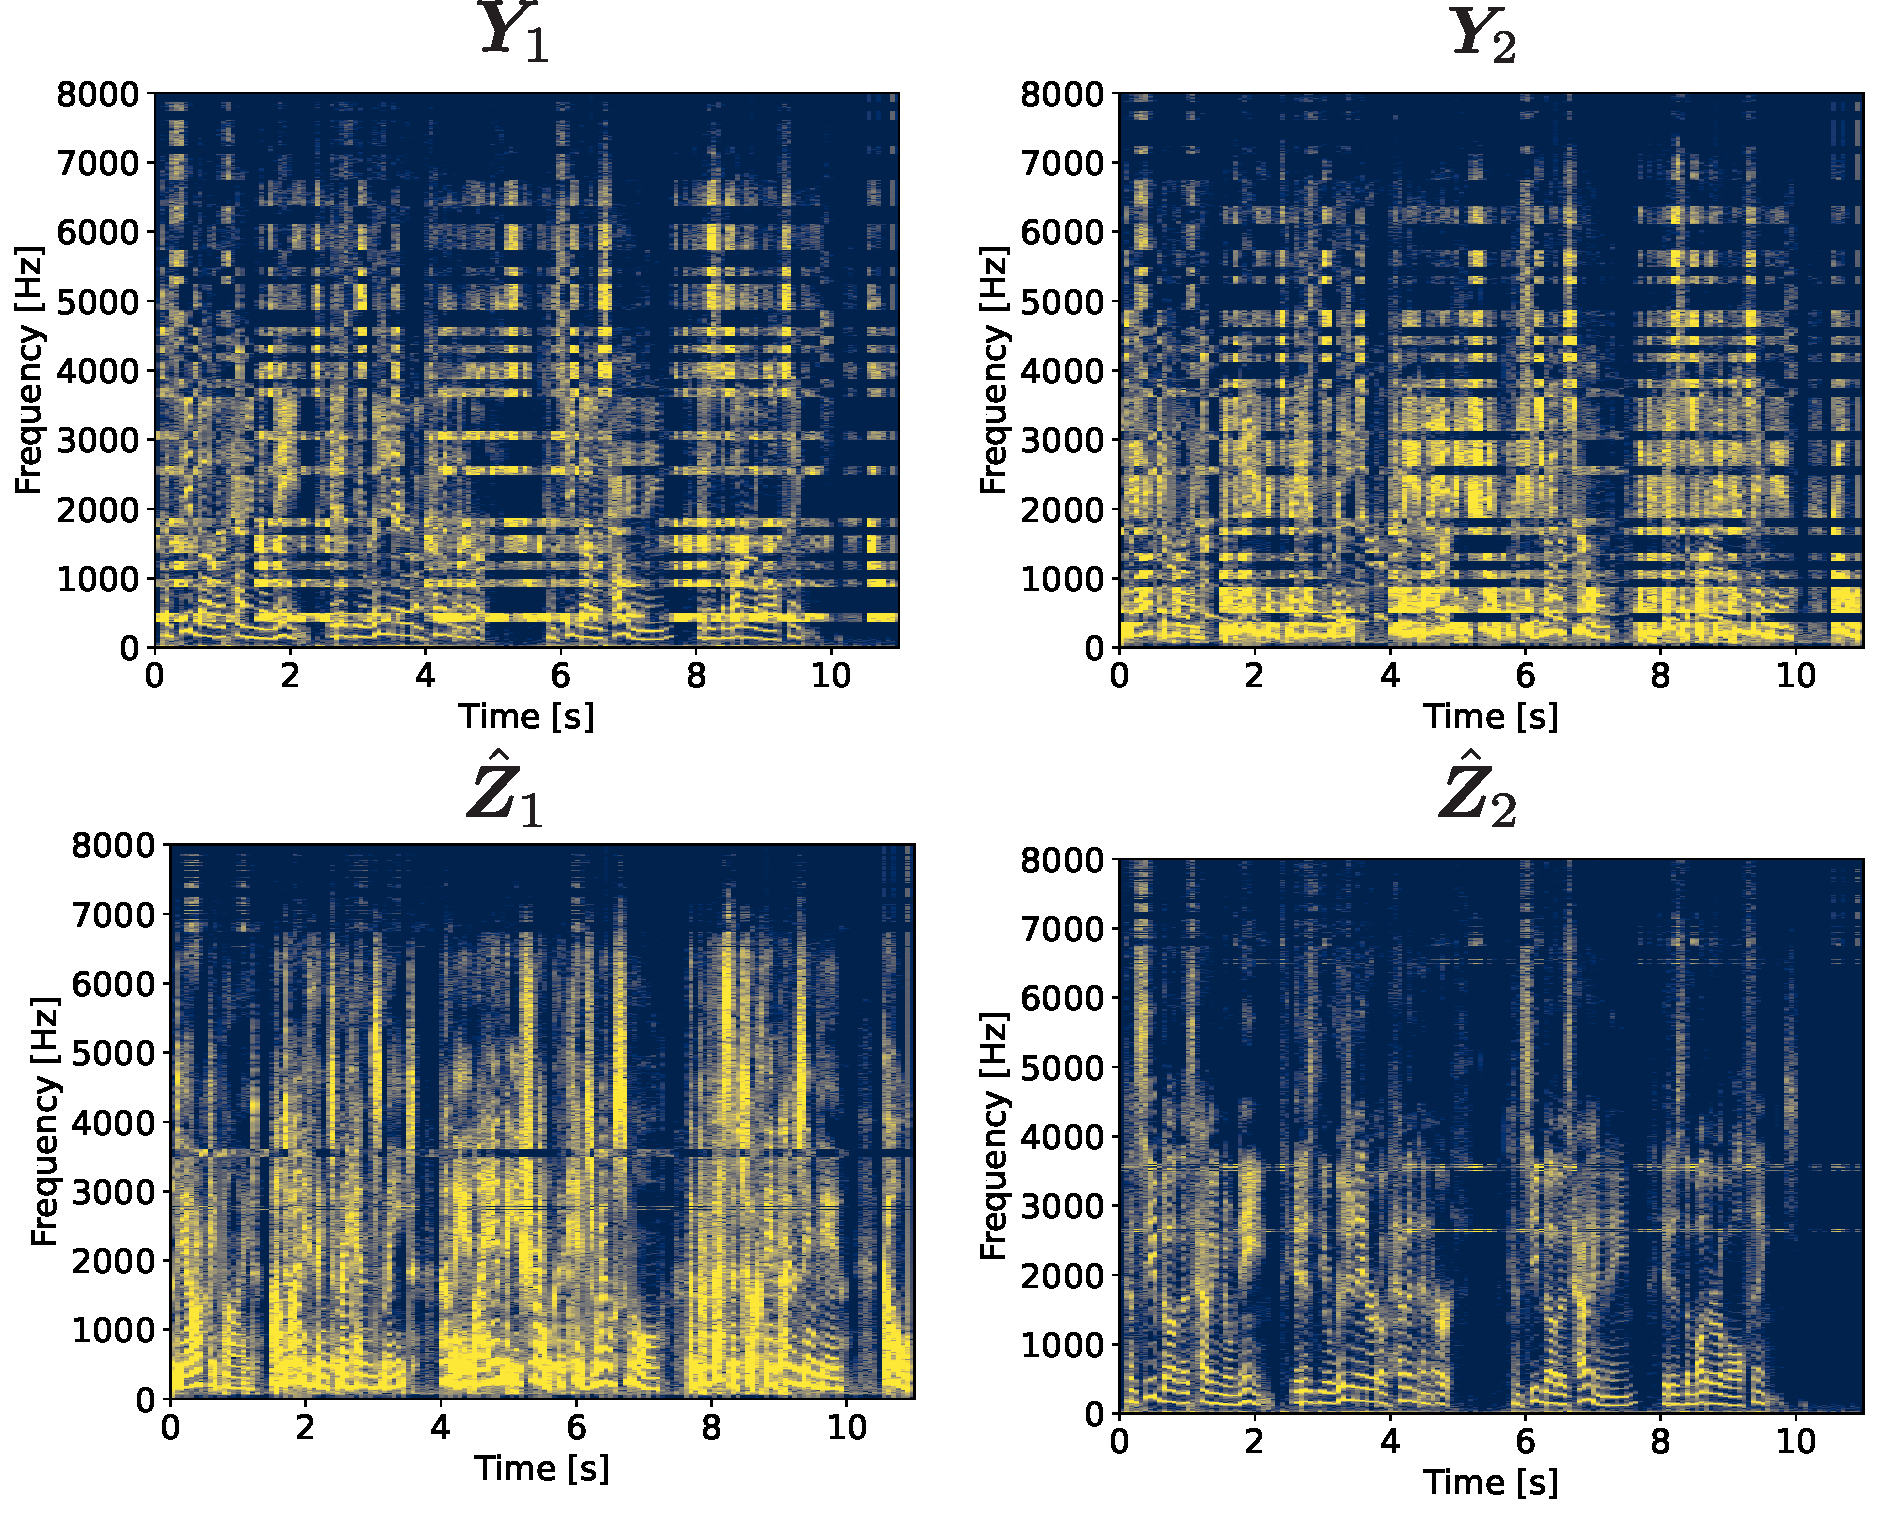
\includegraphics[clip, width=5.0in]{figures/audio_16block.pdf}
  \label{fig:spec_audio_16block}}
  \caption{Experimental results using audio signal of Fig~\ref{fig:audio} (shuffle the frequency every 16 rows).}
  \label{fig:audio_16block}
\end{figure*}
%%%%%%%%%%%%%%%%%%%%%%%%%%%%

%%%%%%%%%%%%%%%%%%%%%%%%%%%%
\begin{figure*}[!t]
  \centering
  \subfloat[Percentage of correct answers for training and validation data.]{\includegraphics[clip, width=4.5in]{figures/graph/Drum_16block.pdf}
  \label{fig:acc_Drum_16block}}
  \\
  \subfloat[Spectrogram of estimated signal and predictive separation signal.]{\includegraphics[clip, width=5.0in]{figures/Drum_16block.pdf}
  \label{fig:spec_Drum_16block}}  
  \caption{Experimental results using instrumental sound of Fig~\ref{fig:drum} (shuffle the frequency every 16 rows).}
  \label{fig:Drum_16block}
\end{figure*}
%%%%%%%%%%%%%%%%%%%%%%%%%%%%

Fig.~\ref{fig:audio_16block}は音声信号を用いた時の結果であり,Fig.~\ref{fig:Drum_16block}は楽器音を用いた時の結果である.
音声信号,楽器音のどちらに対しても,検証データの正答率が90\%を超えており,$\hat{\bm{Z}}_1$,$\hat{\bm{Z}}_2$を概ね的確に推定することができていることが分かる.
従って,ある程度の塊毎に各周波数成分のシャッフルが行われているときは,実際の音声信号や楽器音でもDNNは高精度で分離信号を予測することが可能であるといえる.

\clearpage
%----------------------------------------------
\section{本章のまとめ}
\label{sec:matome}
%----------------------------------------------
本章では,提案手法の有効性を確認するため,人工的に作成したデータと実際の音声及び音楽信号を用意し実験を行った.
実験の結果より,人工データを用いたブロック単位でのパーミュテーション問題に対しては,どのような行列であっても100\%に近い確率で解決できることを示した.
実際の音声データに対しても,ブロック単位でシャッフルが行われていると90\%を超える正答率になることを示した.
次章では,本論文における総括とした結論を述べる.
